%%================================================
%% Filename: chap03.tex
%% Encoding: UTF-8
%% Author: Yuan Xiaoshuai - yxshuai@gmail.com
%% Created: 2012-04-27 19:47
%% Last modified: 2019-11-07 14:38
%%================================================
\chapter{基于数据包标记溯源的模型防护方法}
\chapter{基于数据包标记溯源的模型防护方法}
% \chapter{基于接口号分组的概率标记法}
\label{cha:IGPPM}

在前章中,本文构建了一个多模态特征融合模型,并通过实验验证了该模型的优越性。
随后,本文又为此模型实现了增量学习机制,以便模型能够灵活适应不断变化的网络攻击环境。
然而,在模型的实际运行过程中,很可能会遭遇DDoS攻击的威胁,尤其是当攻击者采用伪造IP地址并频繁更换时,单纯依赖封锁IP的方式难以有效过滤攻击流量。
这种情况下,模型很可能会负担过重,甚至面临崩溃的风险。
针对这一问题,本文将提出一种针对攻击流量进行源头过滤的防护方法,旨在从攻击流量的源头处阻断攻击流量,保护模型的稳定运行。
图~\ref{fig:overall_structure}~是该方法的具体流程。
\begin{figure}[h]
	\centering
	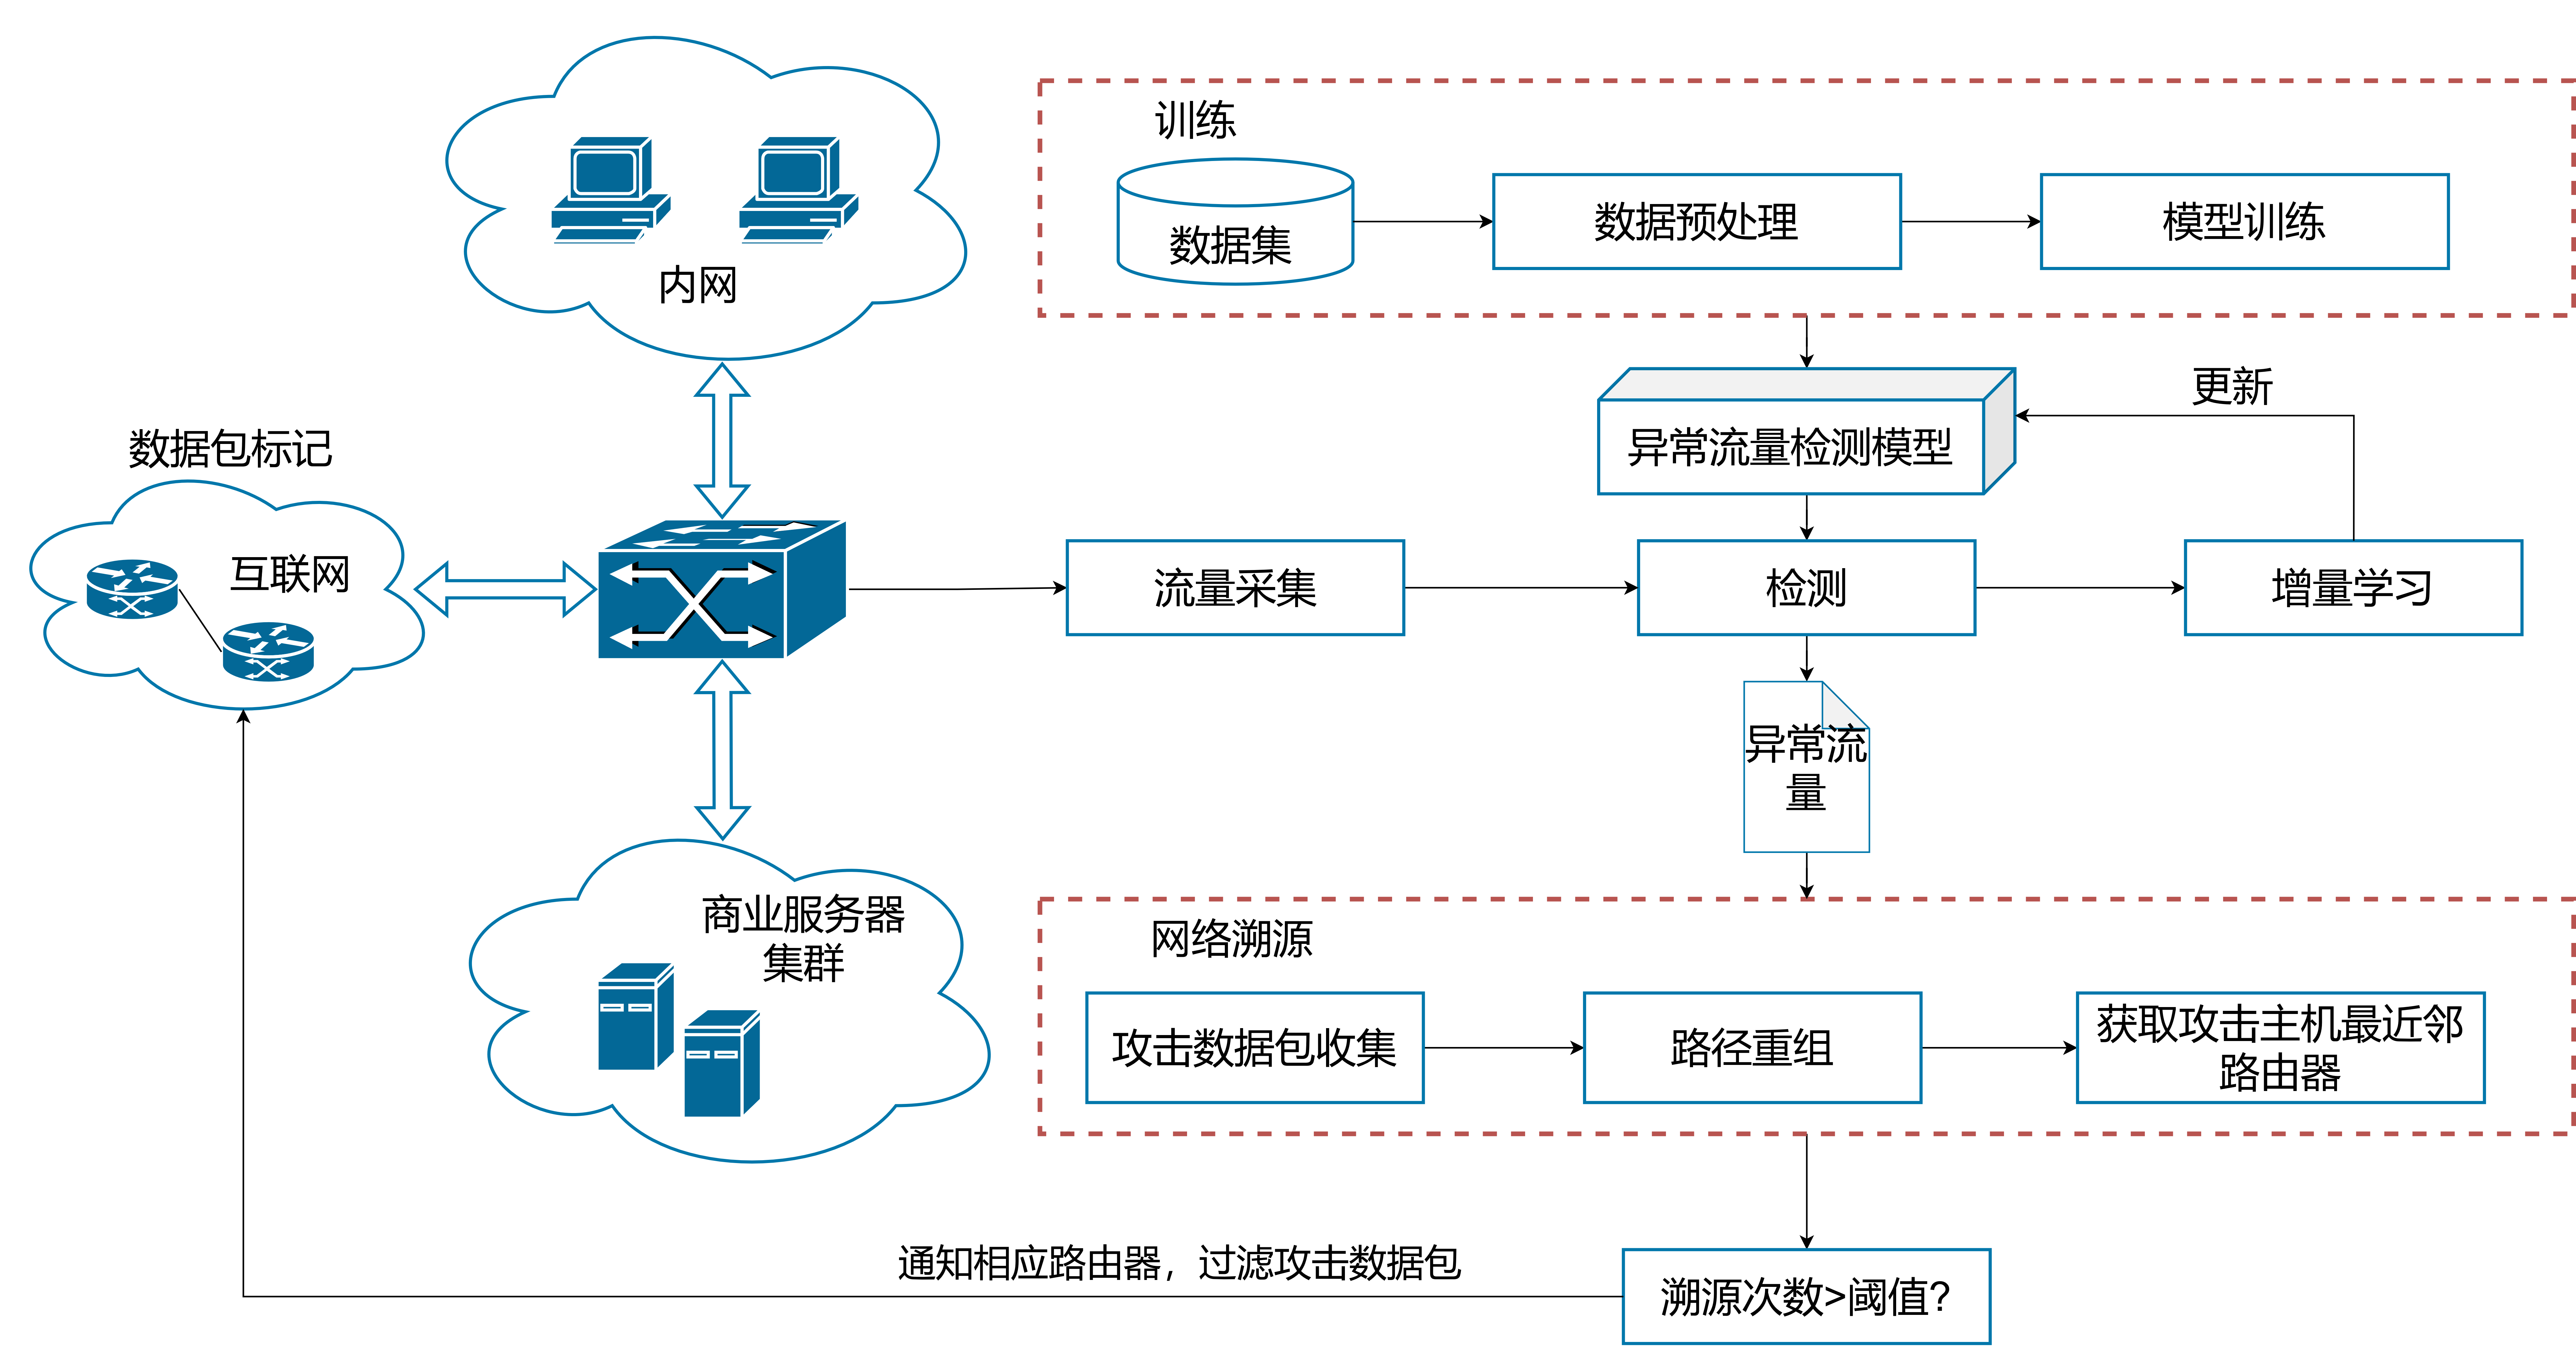
\includegraphics[width = \textwidth]{overall_structure.drawio.png}
	\caption{防护方法具体流程}
	\label{fig:overall_structure}
\end{figure}
该方法的核心在于精确溯源攻击流量,确定距离攻击者最近的路由器,并依托该路由器阻断攻击流量的传播。
这样做的原因有二:一是为定位攻击者提供关键线索;二是尽量减少受阻断流量传播影响的用户数量。\par

因此,要实现该防护方法首先就需要一个行之有效的溯源方法。
数据包标记溯源方法具有简单、高效准确的优点,因此本文将基于其原理,提出一种基于路由器接口号成组标记的数据包标记溯源方法作为防护方法的核心支撑。
该溯源方法以路由器接口号作为标记信息,相比传统数据包标记法依赖IP地址的方式,显著降低了对单个路由信息进行标记所需的存储空间。
此外,该溯源方法通过结合异或运算的特性,不仅确保了溯源的准确率,而且显著提升了路径重构的速度,从而实现了高效且准确的溯源过程。

在前章中,本文构建了一个多模态特征融合模型,并通过实验验证了该模型的优越性。
随后,本文又为此模型实现了增量学习机制,以便模型能够灵活适应不断变化的网络攻击环境。
然而,在模型的实际运行过程中,很可能会遭遇DDoS攻击的威胁,尤其是当攻击者采用伪造IP地址并频繁更换时,单纯依赖封锁IP的方式难以有效过滤攻击流量。
这种情况下,模型很可能会负担过重,甚至面临崩溃的风险。
针对这一问题,本文将提出一种针对攻击流量进行源头过滤的防护方法,旨在从攻击流量的源头处阻断攻击流量,保护模型的稳定运行。
图~\ref{fig:overall_structure}~是该方法的具体流程。
\begin{figure}[h]
	\centering
	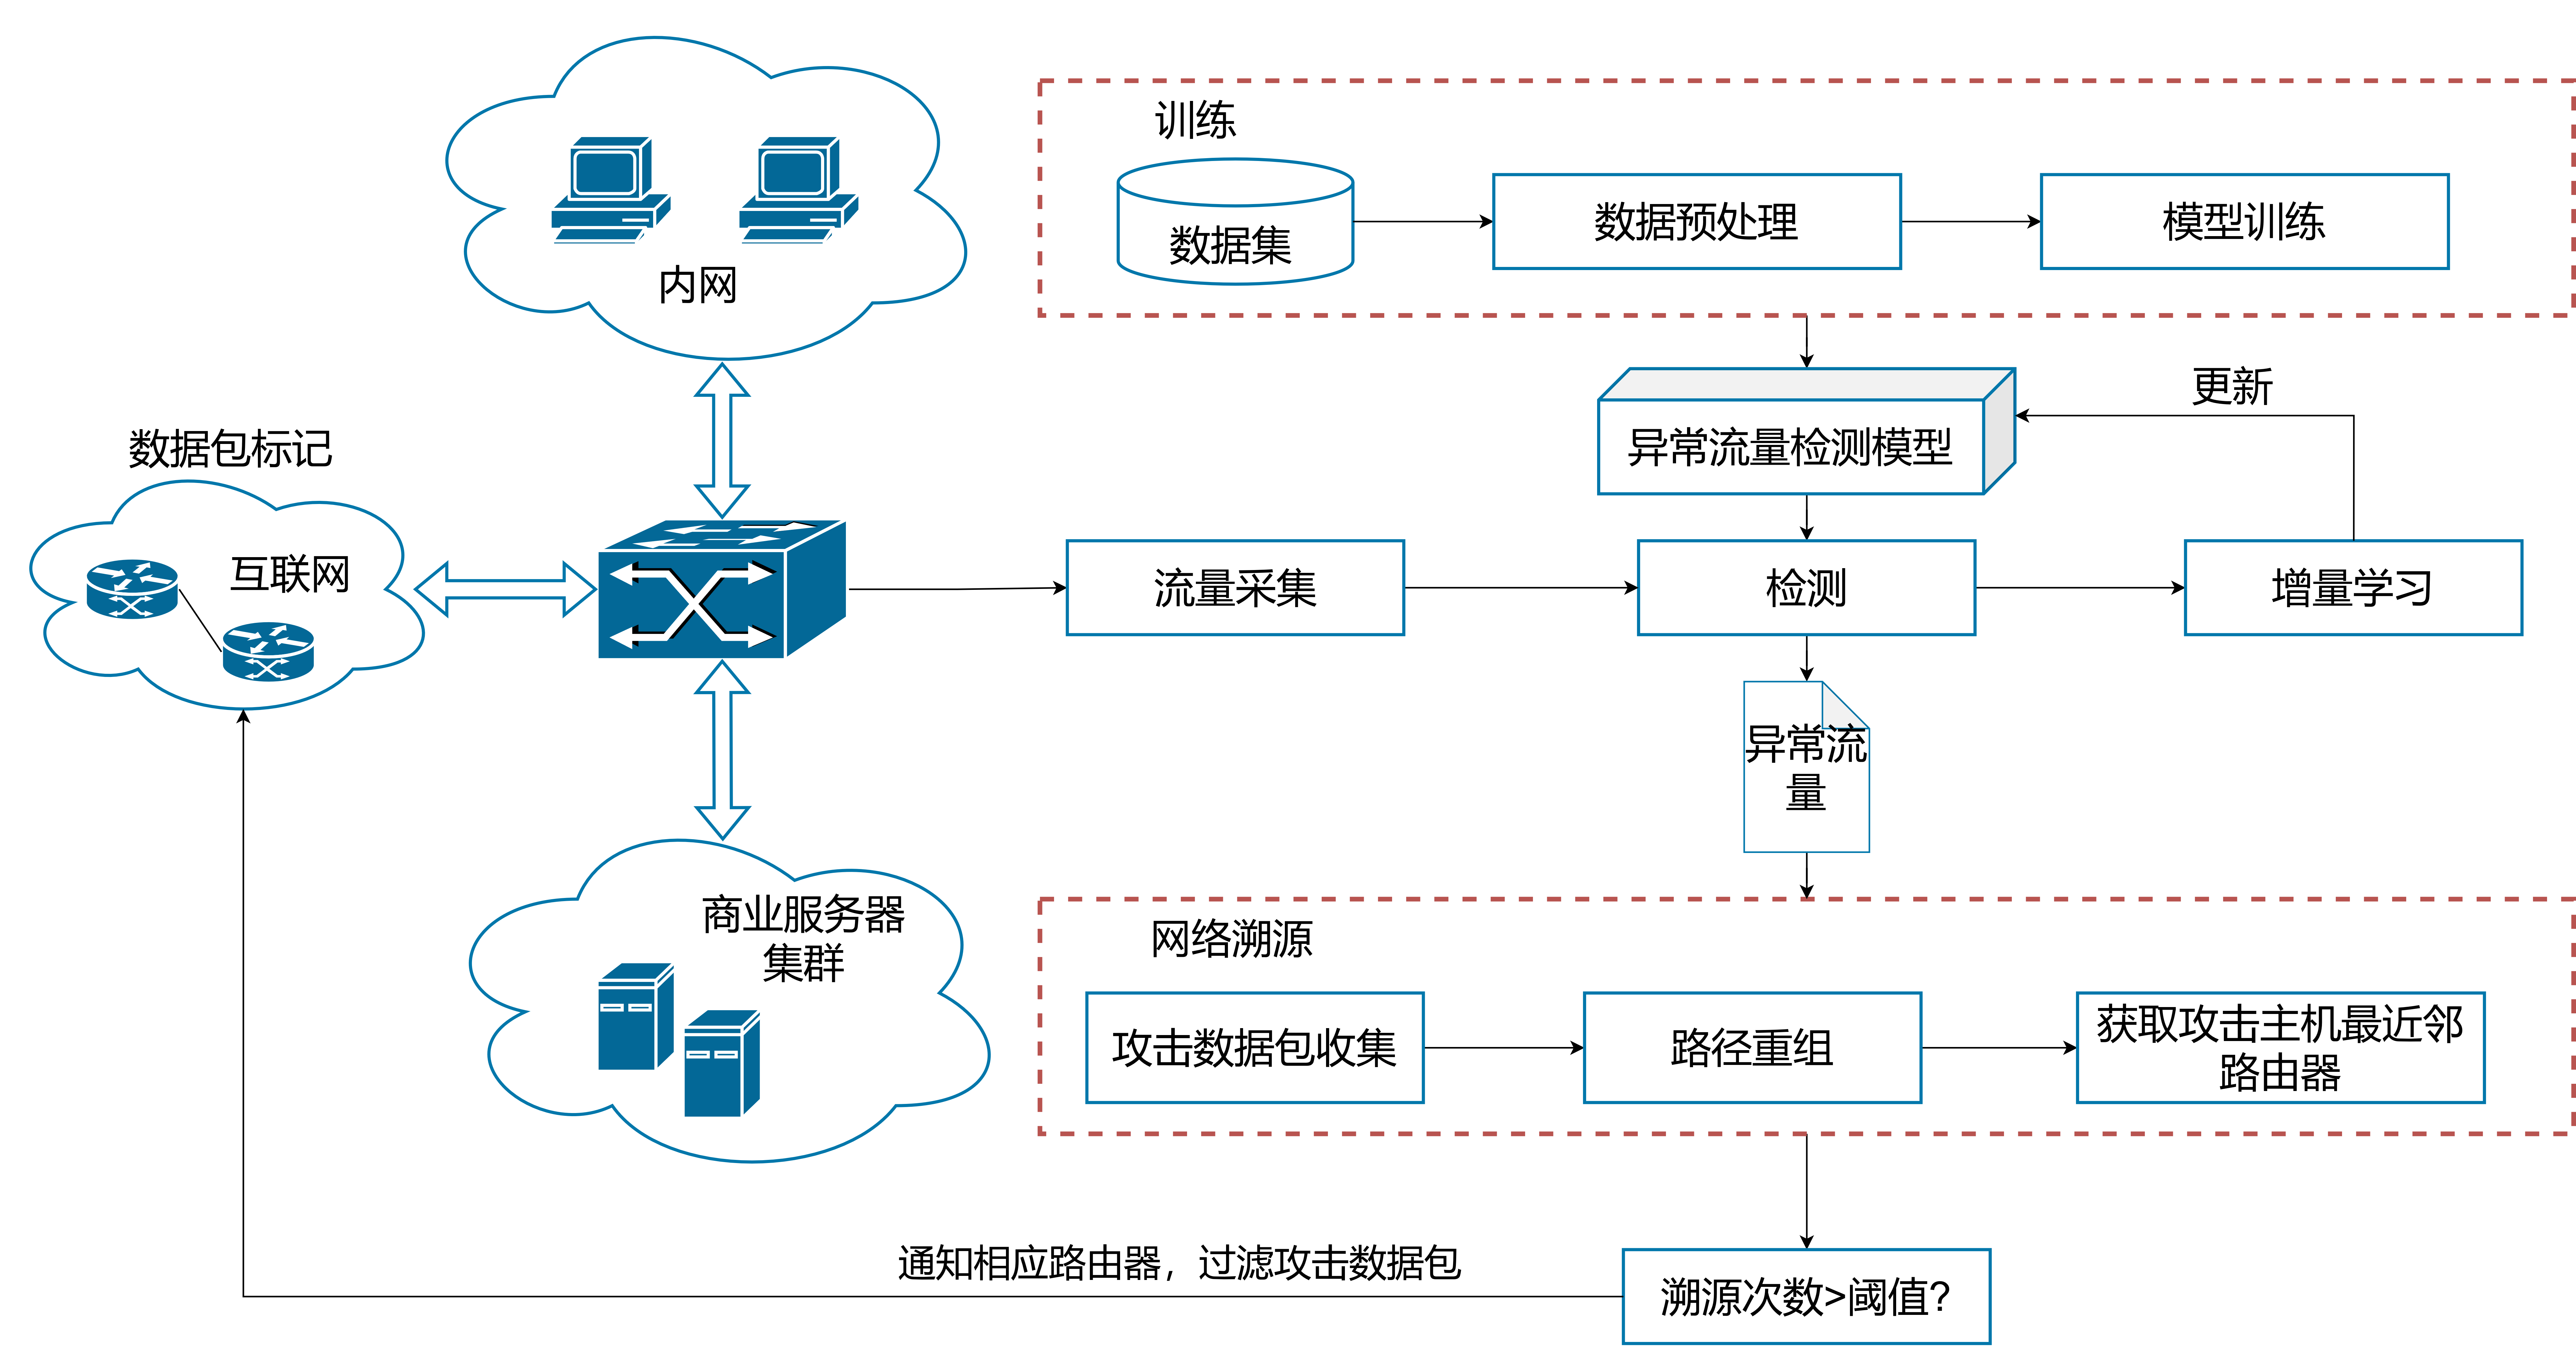
\includegraphics[width = \textwidth]{overall_structure.drawio.png}
	\caption{防护方法具体流程}
	\label{fig:overall_structure}
\end{figure}
该方法的核心在于精确溯源攻击流量,确定距离攻击者最近的路由器,并依托该路由器阻断攻击流量的传播。
这样做的原因有二:一是为定位攻击者提供关键线索;二是尽量减少受阻断流量传播影响的用户数量。\par

因此,要实现该防护方法首先就需要一个行之有效的溯源方法。
数据包标记溯源方法具有简单、高效准确的优点,因此本文将基于其原理,提出一种基于路由器接口号成组标记的数据包标记溯源方法作为防护方法的核心支撑。
该溯源方法以路由器接口号作为标记信息,相比传统数据包标记法依赖IP地址的方式,显著降低了对单个路由信息进行标记所需的存储空间。
此外,该溯源方法通过结合异或运算的特性,不仅确保了溯源的准确率,而且显著提升了路径重构的速度,从而实现了高效且准确的溯源过程。

\section{基于路由器接口号成组标记的溯源方法}
\section{基于路由器接口号成组标记的溯源方法}

基于路由器接口号成组标记的溯源方法旨在当模型检测到攻击流量时,实现高效、精准的溯源,以便防护方法从源头上过滤攻击流量,确保模型正常稳定运行。
该溯源方法主要分为三个阶段:路由器标记阶段、标记数据包收集阶段、路径重组阶段。
基于路由器接口号成组标记的溯源方法旨在当模型检测到攻击流量时,实现高效、精准的溯源,以便防护方法从源头上过滤攻击流量,确保模型正常稳定运行。
该溯源方法主要分为三个阶段:路由器标记阶段、标记数据包收集阶段、路径重组阶段。
这三个阶段如图~\ref{fig:our_datapackets_design}~所示。
\begin{figure}[h]
	\centering
	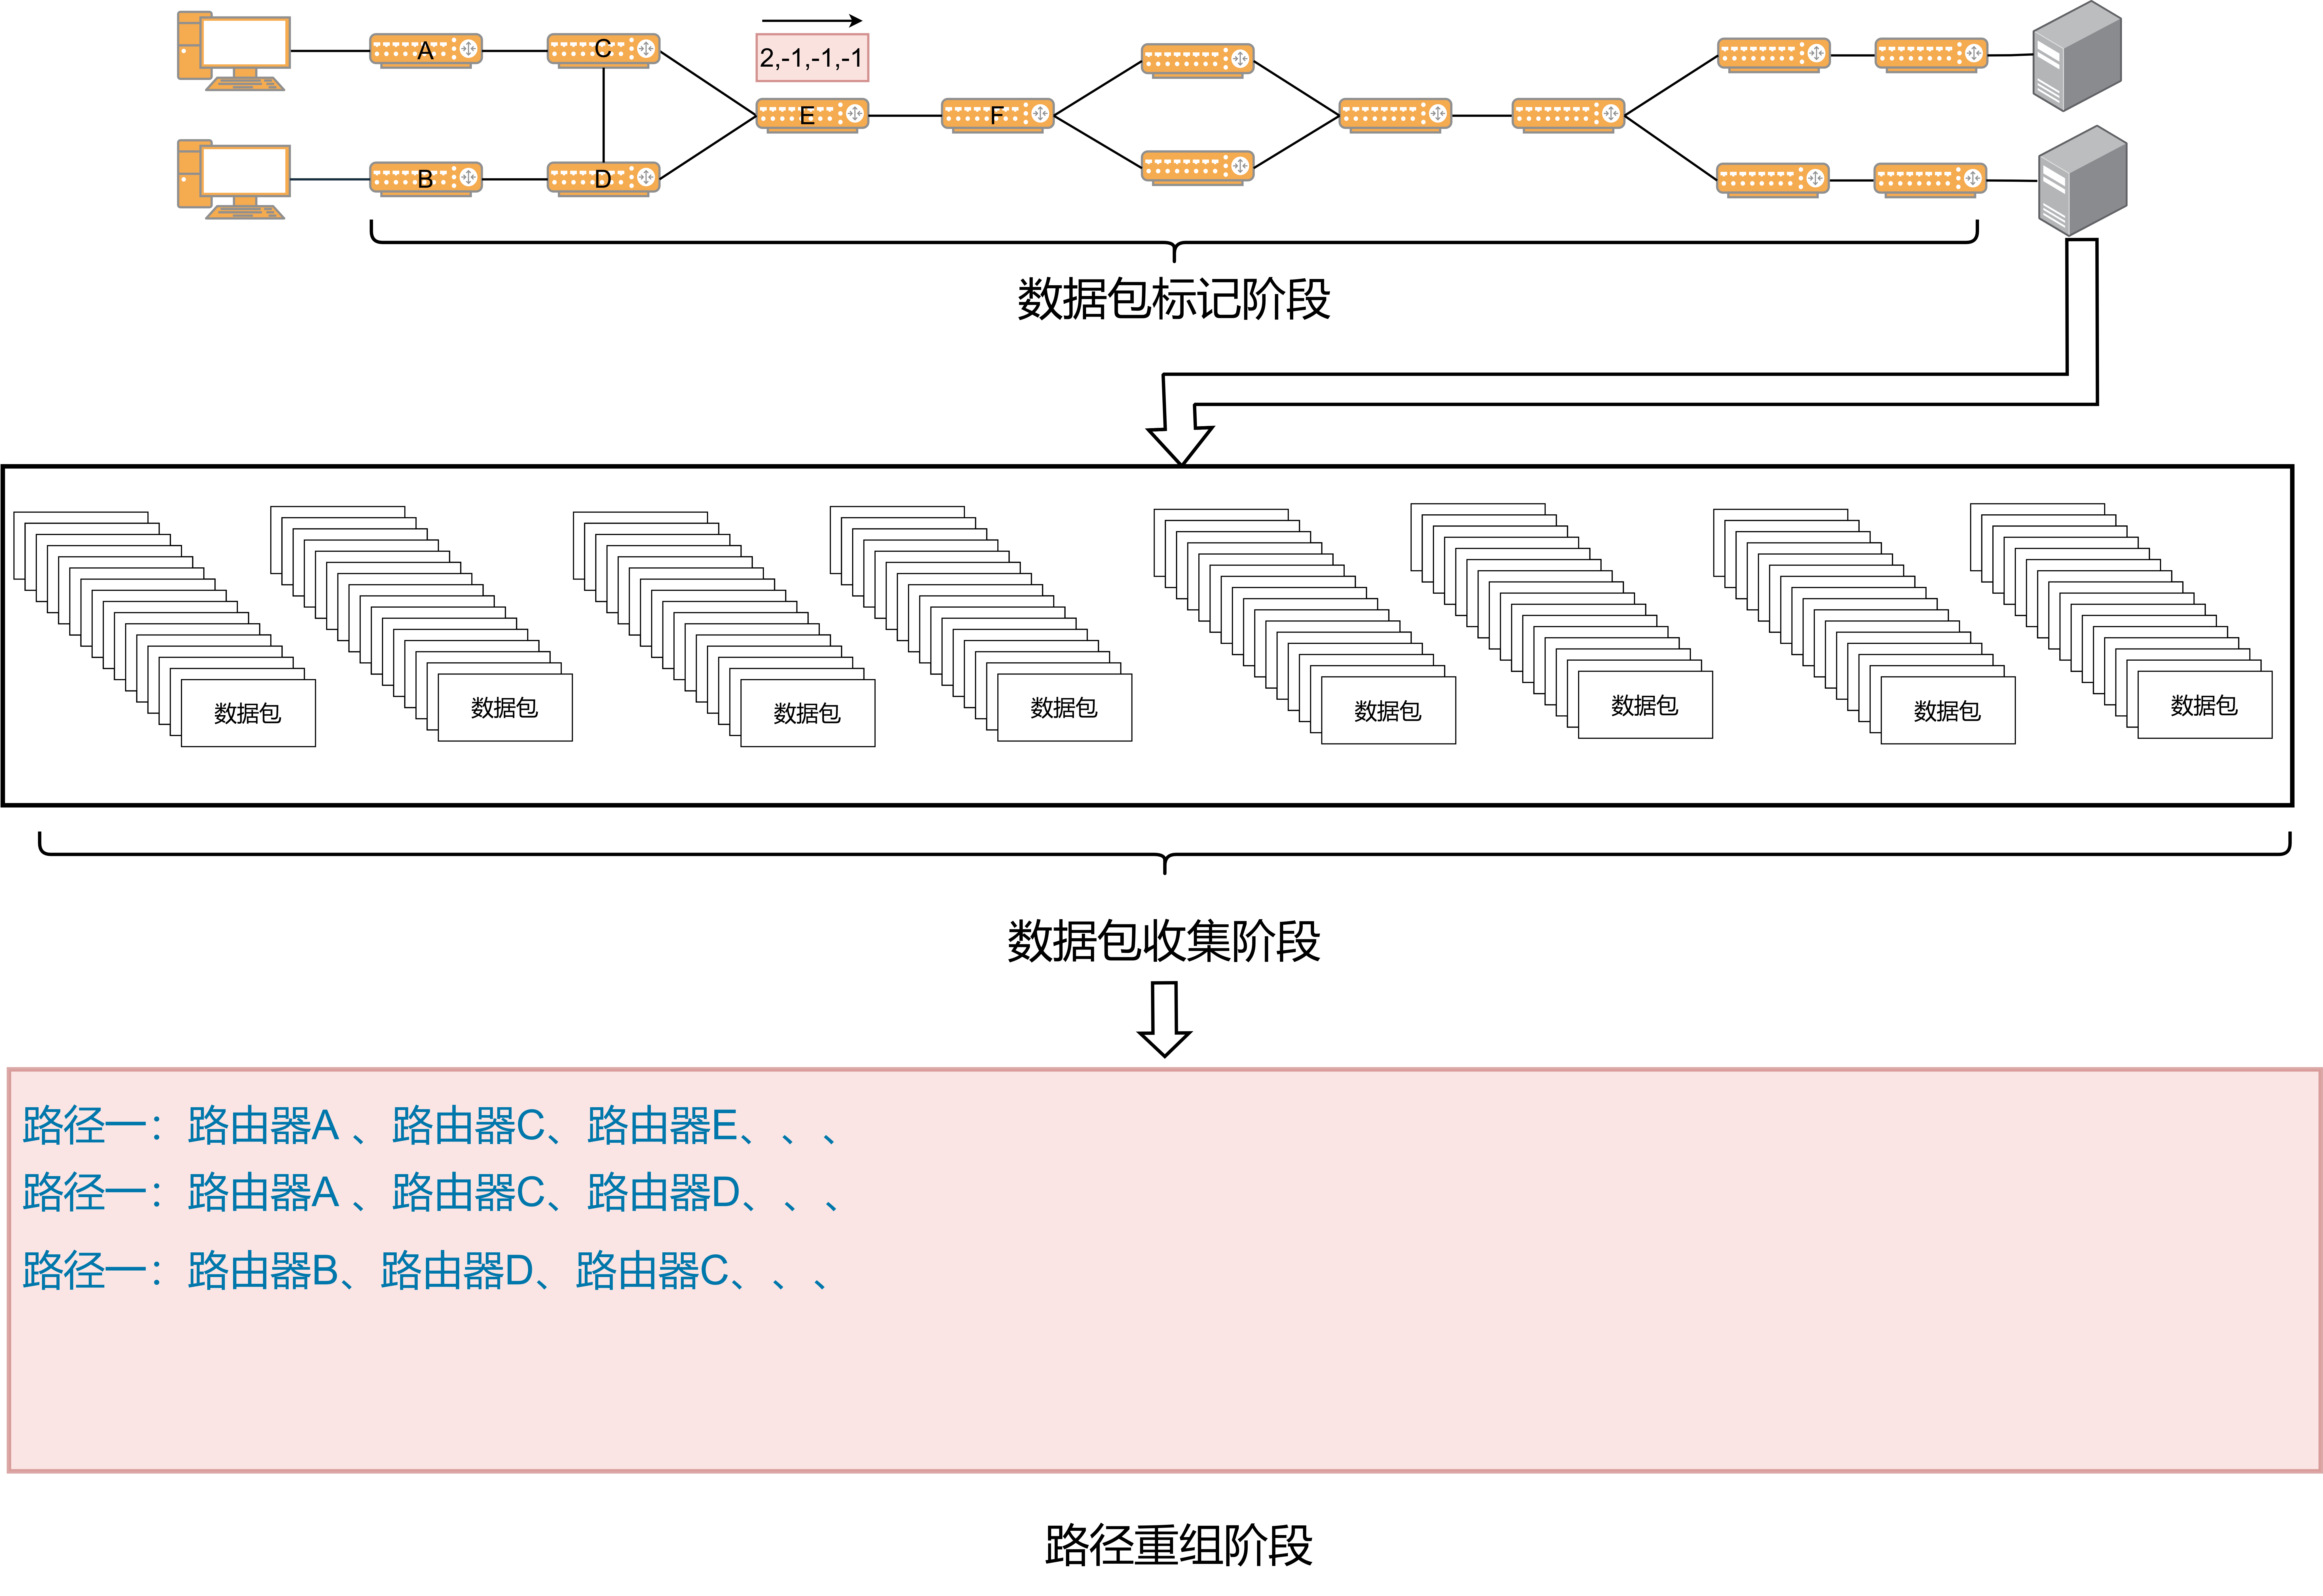
\includegraphics[width = \textwidth]{datapackets.drawio.png}
	\caption{基于接口号分组的概率标记溯源法流程}
	\label{fig:our_datapackets_design}
	\centering
	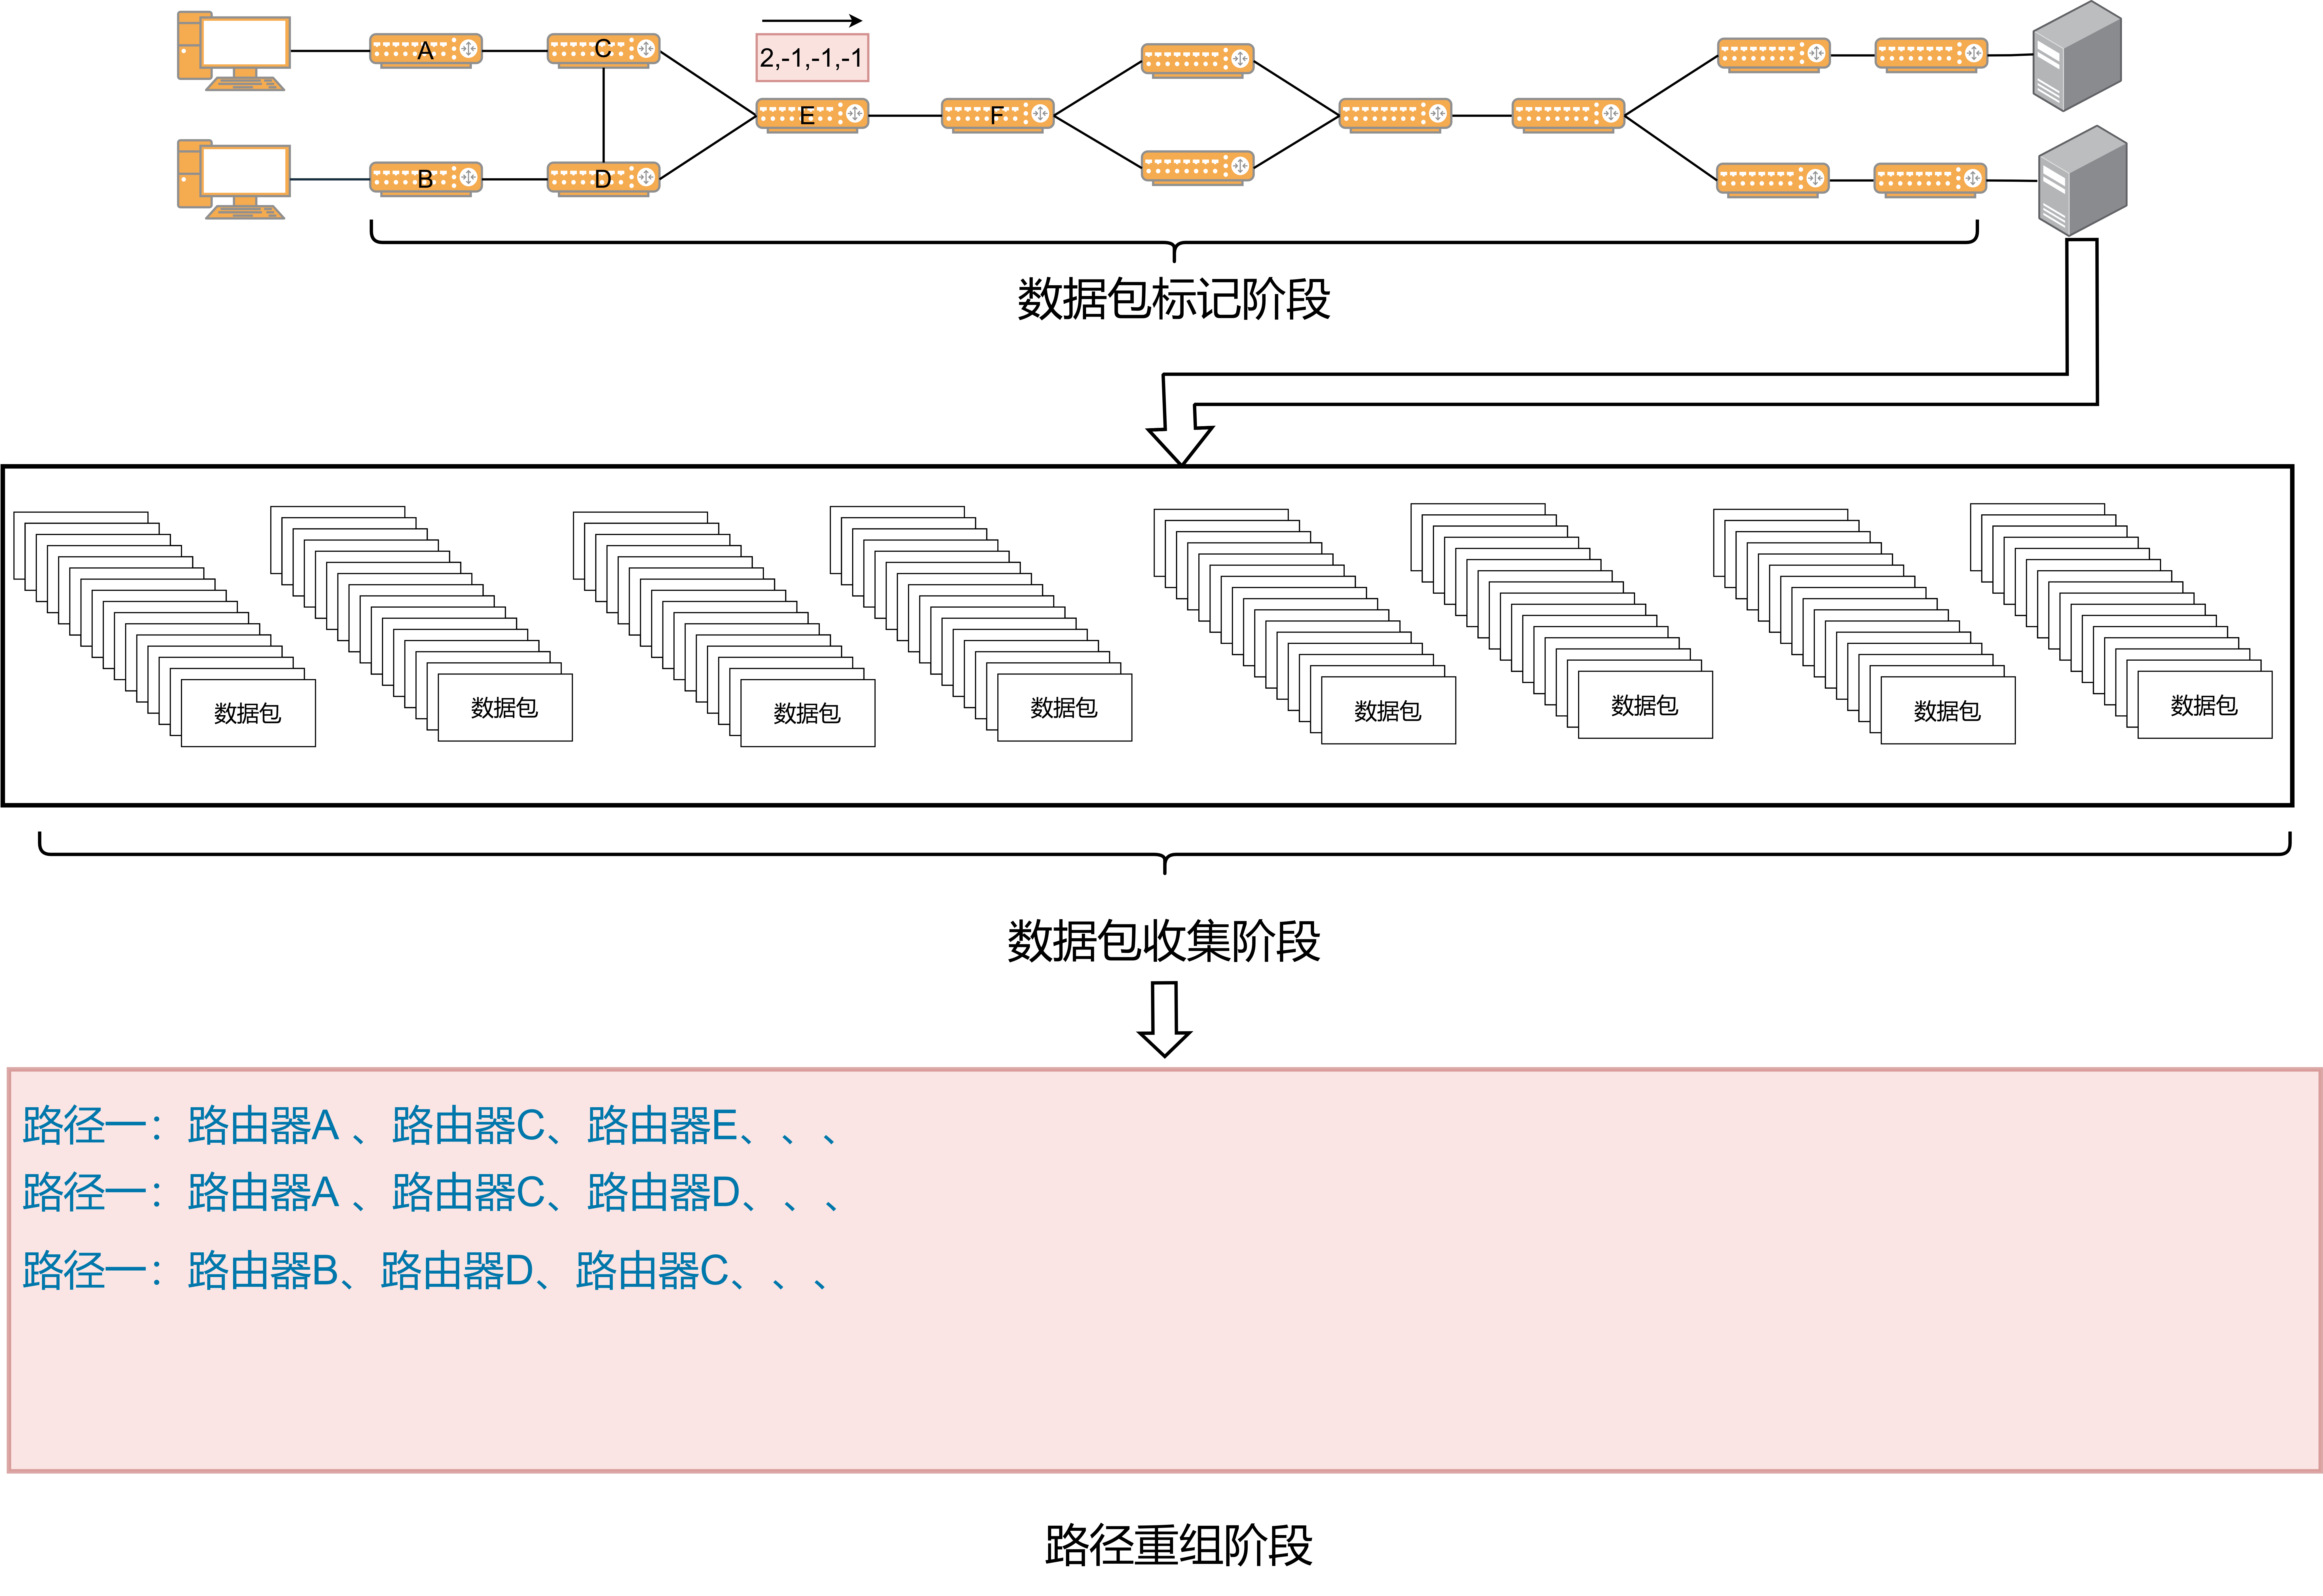
\includegraphics[width = \textwidth]{datapackets.drawio.png}
	\caption{基于接口号分组的概率标记溯源法流程}
	\label{fig:our_datapackets_design}
\end{figure}
首先是数据包标记阶段,它是网络追踪的起始步骤,发生在数据包于网络路径上的传输过程中。
当数据包离开发送者设备进入网络后,中间路由器便会根据预设策略对经过的数据包进行概率性标记,将路由器获取到该数据包的接口号写入到本文接下来将要提出的标记信息结构体中,以便路径重构程序有效利用这些信息准确完成路径重构。
当数据包离开发送者设备进入网络后,中间路由器便会根据预设策略对经过的数据包进行概率性标记,将路由器获取到该数据包的接口号写入到本文接下来将要提出的标记信息结构体中,以便路径重构程序有效利用这些信息准确完成路径重构。

其次是标记数据包收集阶段,这一环节主要在受害者服务器上进行。
一旦运行在受害者服务器上的异常流量检测模型识别到异常流量,便会立即启动收集机制,专门对携带标记信息的攻击数据包进行收集。
一旦运行在受害者服务器上的异常流量检测模型识别到异常流量,便会立即启动收集机制,专门对携带标记信息的攻击数据包进行收集。
值得注意的是,这一收集过程与路由器标记阶段可以并行进行,从而提高追踪效率。

当服务器成功收集到足够数量的标记数据包后,便进入路径重组阶段。
在这一阶段,通过利用服务器所收集到的带有标记信息的攻击数据包,执行路径重构算法,便能够得到一条条有序的路由器接口号序列,即接口号路径。
之后服务器可根据此接口号路径对路由器进行递归查询,便能够查询到距离攻击源的“最近邻路由器”,至此便完成一个完整的溯源任务。
最后,服务器可实时监控并统计一段时间内该路由器被溯源到的次数,一旦该次数超过预设的阈值,服务器将立即采取行动,通知该路由器停止转发目标地址为服务器IP的数据包。
接下来,本节将首先提出一种专门用于记录数据包标记信息的结构体,随后会围绕前述提到的三个关键阶段对本文所提出的溯源方案展开详细叙述。
\subsection{标记信息结构体:MarkInfo}
在这一阶段,通过利用服务器所收集到的带有标记信息的攻击数据包,执行路径重构算法,便能够得到一条条有序的路由器接口号序列,即接口号路径。
之后服务器可根据此接口号路径对路由器进行递归查询,便能够查询到距离攻击源的“最近邻路由器”,至此便完成一个完整的溯源任务。
最后,服务器可实时监控并统计一段时间内该路由器被溯源到的次数,一旦该次数超过预设的阈值,服务器将立即采取行动,通知该路由器停止转发目标地址为服务器IP的数据包。
接下来,本节将首先提出一种专门用于记录数据包标记信息的结构体,随后会围绕前述提到的三个关键阶段对本文所提出的溯源方案展开详细叙述。
\subsection{标记信息结构体:MarkInfo}
路由器对数据包进行标记的过程,实质上就是路由器将自身的信息写入到数据包的过程。
数据包在网络路径上传输时,可能会经历多个这样的标记过程,直至最终抵达服务器。
对于服务器而言,要完成路径重构,就必须从数据包中提取并分析这些标记过程产生的信息以及这些信息的关系。
对于服务器而言,要完成路径重构,就必须从数据包中提取并分析这些标记过程产生的信息以及这些信息的关系。
因此,如何在数据包中有效组织并存储这些信息及其关系显得尤为重要。
基于这一需求,本文设计并提出了一种专门在数据包中存储和组织这些标记信息的结构体(如图~\ref{fig:data_structure}~所示):MarkInfo。

\begin{figure}[h]
	\centering
	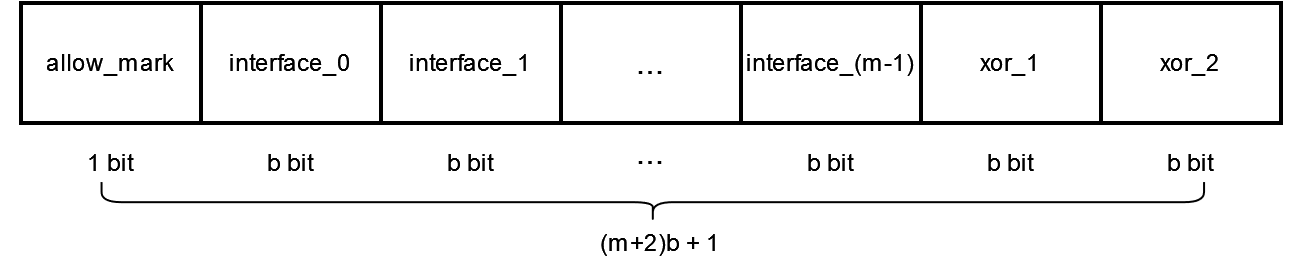
\includegraphics[width = 0.8\textwidth]{markinfo.drawio.png}
	\caption{本文所设计的用于在数据包中记录标记信息的结构体}
	\label{fig:data_structure}
\end{figure}
	\centering
	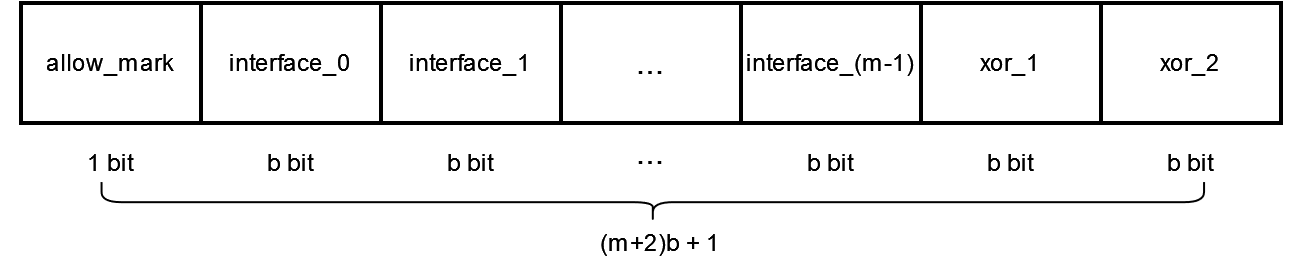
\includegraphics[width = 0.8\textwidth]{markinfo.drawio.png}
	\caption{本文所设计的用于在数据包中记录标记信息的结构体}
	\label{fig:data_structure}
\end{figure}

该结构体共由三类字段组成。
首先,是允许标志位(allow\_mark),长度为1 bit。
这一字段的作用是控制后续路由器能否对数据包进行概率标记。
若值为0,则所有路由器均不对该数据包进行标记;若值为1,则后续的组首路由器则会按照预设的概率执行标记操作。
这一设计确保了路径上标记信息的连续性,对于间断式的标记信息,路径重构算法无法有效复原。\par

第二类字段是接口号标记字段(interface\_i),其中i取值范围为[1,m],字段长度为b bit,共可表示$2^b$个接口号。
根据具体的网络环境和溯源需求,b和m的值可灵活调整。
这m个接口号标记字段在路径重构过程中扮演着核心角色。
这m个接口号标记字段在路径重构过程中扮演着核心角色。
每个字段分别记录着数据包在网络传输过程中到达路由器时所经过的输入接口号。


第三类字段则是异或标志位,这类字段共有两个:xor\_1和xor\_2,每个字段与单个接口号标记字段的长度相同。
xor\_1记录的是所有对其标记的路由器输入接口号异或值;
xor\_2则记录数据包从发送者到接收者整条路径上所有路由器输入接口号的异或值,无论是否进行标记。
xor\_1记录的是所有对其标记的路由器输入接口号异或值;
xor\_2则记录数据包从发送者到接收者整条路径上所有路由器输入接口号的异或值,无论是否进行标记。
这两个字段——xor\_2与xor\_1,在后续的路径重构算法中发挥着不可或缺的作用。
xor\_2结合TTL(生存时间)能够有效区分不同的网络传输路径,而xor\_1则可作为一条关键线索,引导路径重构算法的完成。
具体的重构过程将在后续小节中详细阐述。\par
具体的重构过程将在后续小节中详细阐述。\par

总的标记空间大小为 $l = 1 + (m + 2) \times b$ bit,用于支持数据包标记过程。
在实际应用中,可根据具体场景设定b和m的值。
例如,在本文的实验中,考虑到大多数互联网路由器接口数远少于$2^6 =64$个,因此本文设定b = 6。
同时,本文设定了 m 分别为 2 和 4,总共使用了 IP 头部中的 25 和 37 bit,对应标记空间的利用率分别为 0.08 和 0.0108。
在实际应用中,可根据具体场景设定b和m的值。
例如,在本文的实验中,考虑到大多数互联网路由器接口数远少于$2^6 =64$个,因此本文设定b = 6。
同时,本文设定了 m 分别为 2 和 4,总共使用了 IP 头部中的 25 和 37 bit,对应标记空间的利用率分别为 0.08 和 0.0108。
相较于传统使用 IP 地址作为标记信息的策略(利用率为$1/32 \approx 0.0313$),利用率有了显著提高。
通过这样的结构体,本方法能更好的存储数据包在路径传输过程中的收集到的标记信息,方便路径重构算法快速且准确地完成路径重构。\par

\subsection{路由器标记阶段}
通过这样的结构体,本方法能更好的存储数据包在路径传输过程中的收集到的标记信息,方便路径重构算法快速且准确地完成路径重构。\par

\subsection{路由器标记阶段}
路由器的数据包标记过程是以“组”为单位进行的。
因此,本文将数据包从发送者到接收者所经过的整条路径上每连续的m个路由器划分并定义为一个“组”。
因此,本文将数据包从发送者到接收者所经过的整条路径上每连续的m个路由器划分并定义为一个“组”。
其中,距离发送者最近的“组”被定义为“首组”,而距离接收者最近的“组”则为“最后一组”。
值得注意的是,“最后一组”的路由器数量可能少于m个。
假设从发送者到接收者之间共有d跳路由器,那么这d跳路由器可以被划分为k“组”,其中$k=\lceil d/m \rceil$,即向上取整得到组数。
这样的分组方式有助于方案更有效地进行数据包标记和路径重构。\par
当路由器以组为单位对数据包进行概率标记时,第一组的标记概率为1,即直接进行标记,而其余组则以$p \times allow\_mark$概率进行标记(这里,本文假设p为0到1之间的一个小数)。
另外,需要注意的是,具体的概率判定组是否标记是由组首路由器完成的。\par
图~\ref{fig:marking_procedure}~是标记操作的详细流程图。
\begin{figure}[h]
	\centering
	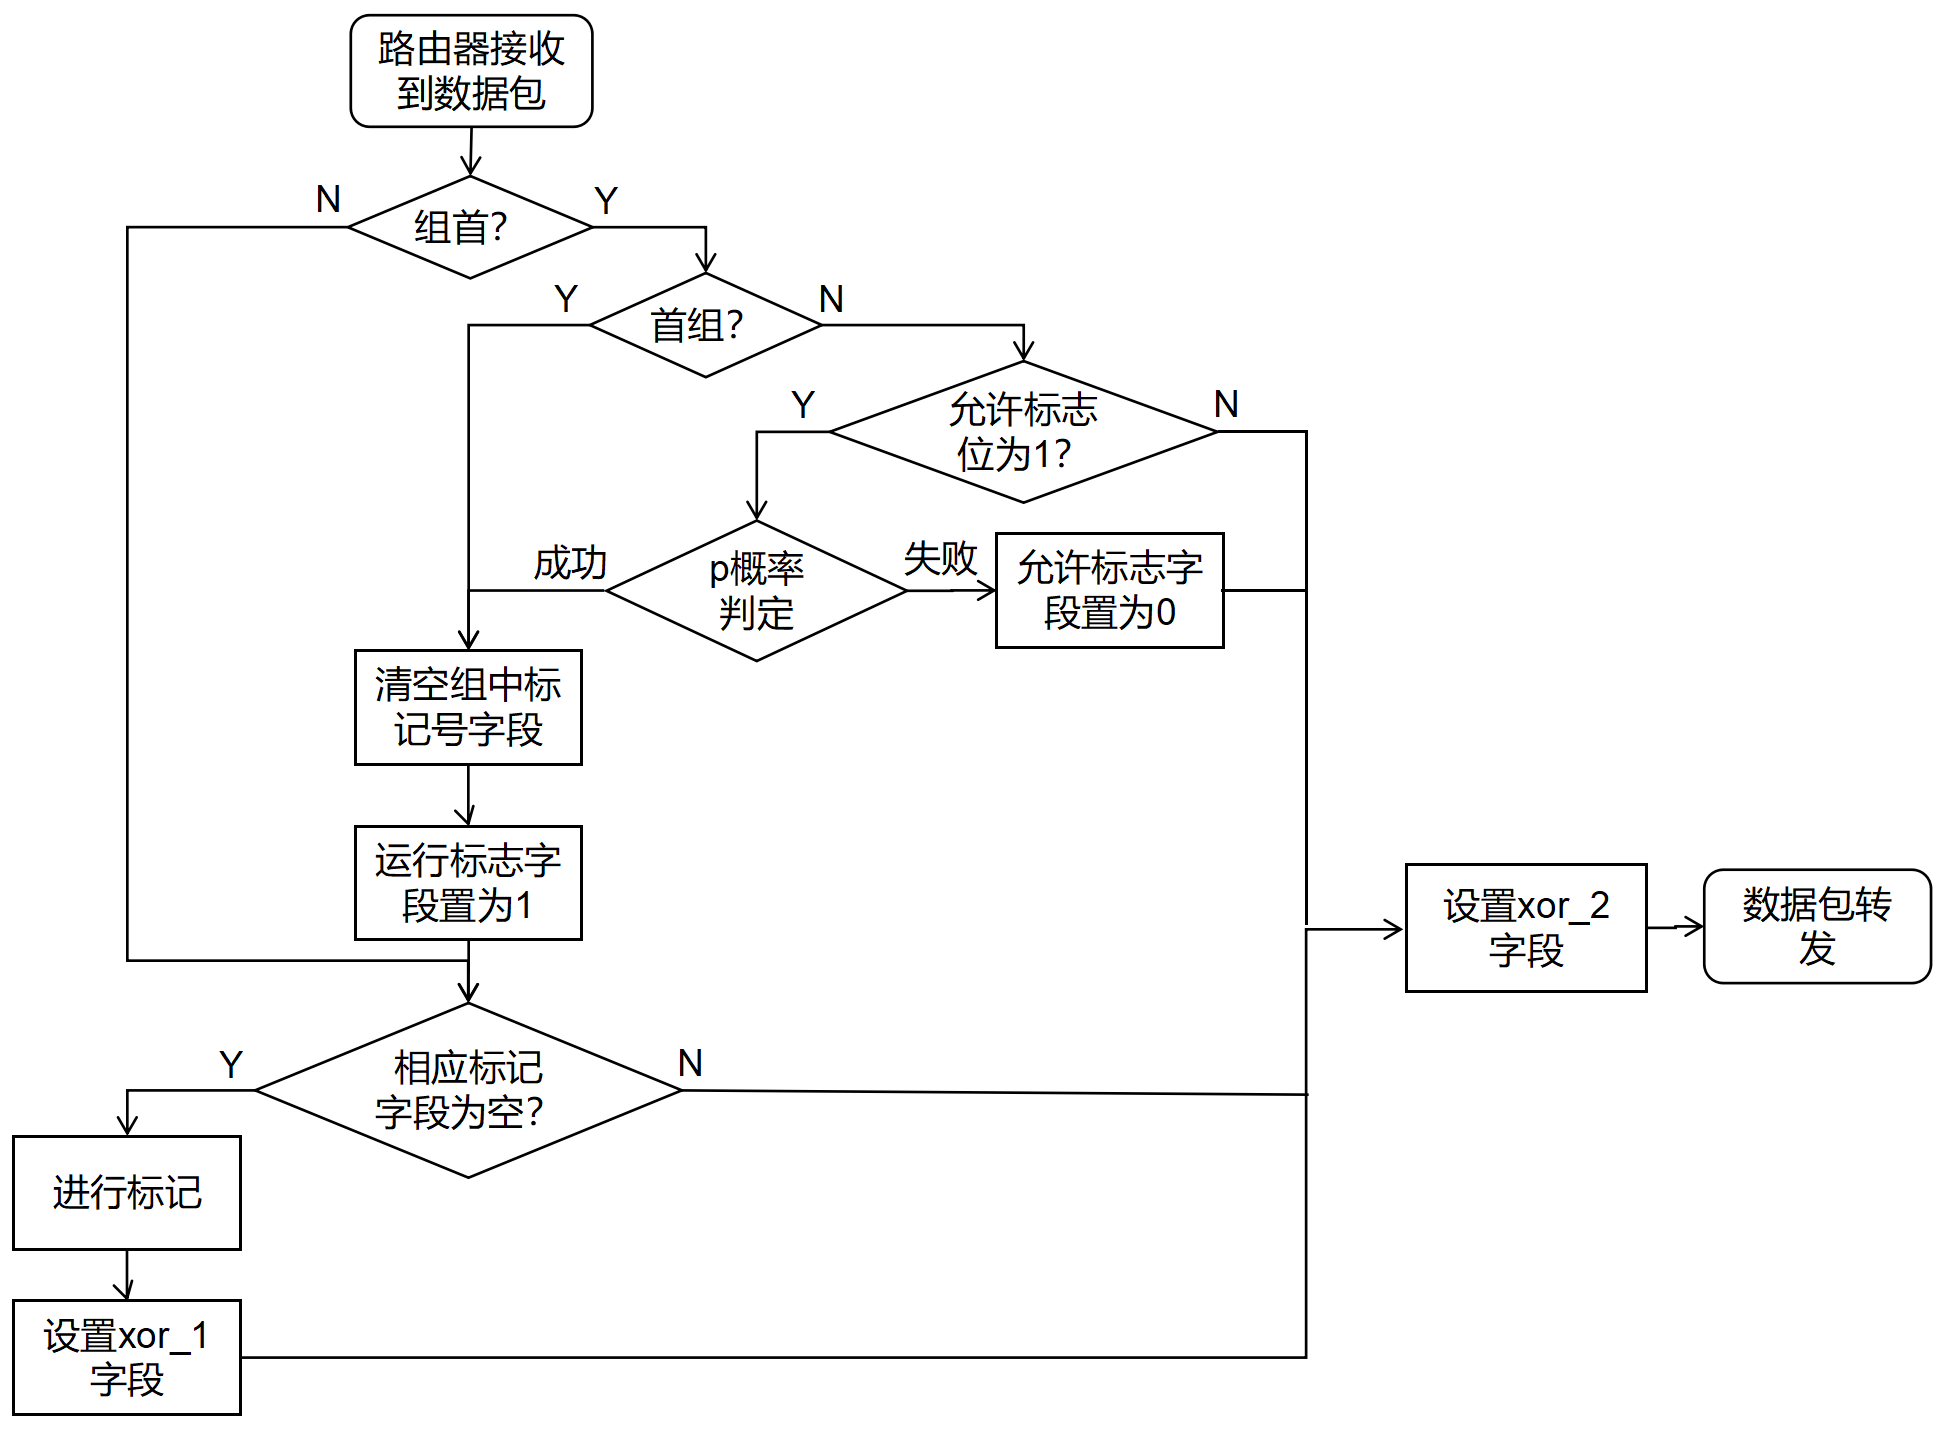
\includegraphics[width = 0.9\textwidth]{marking_procedure.png}
	\caption{路由器标记操作流程图}
	\label{fig:marking_procedure}
\end{figure}
	\centering
	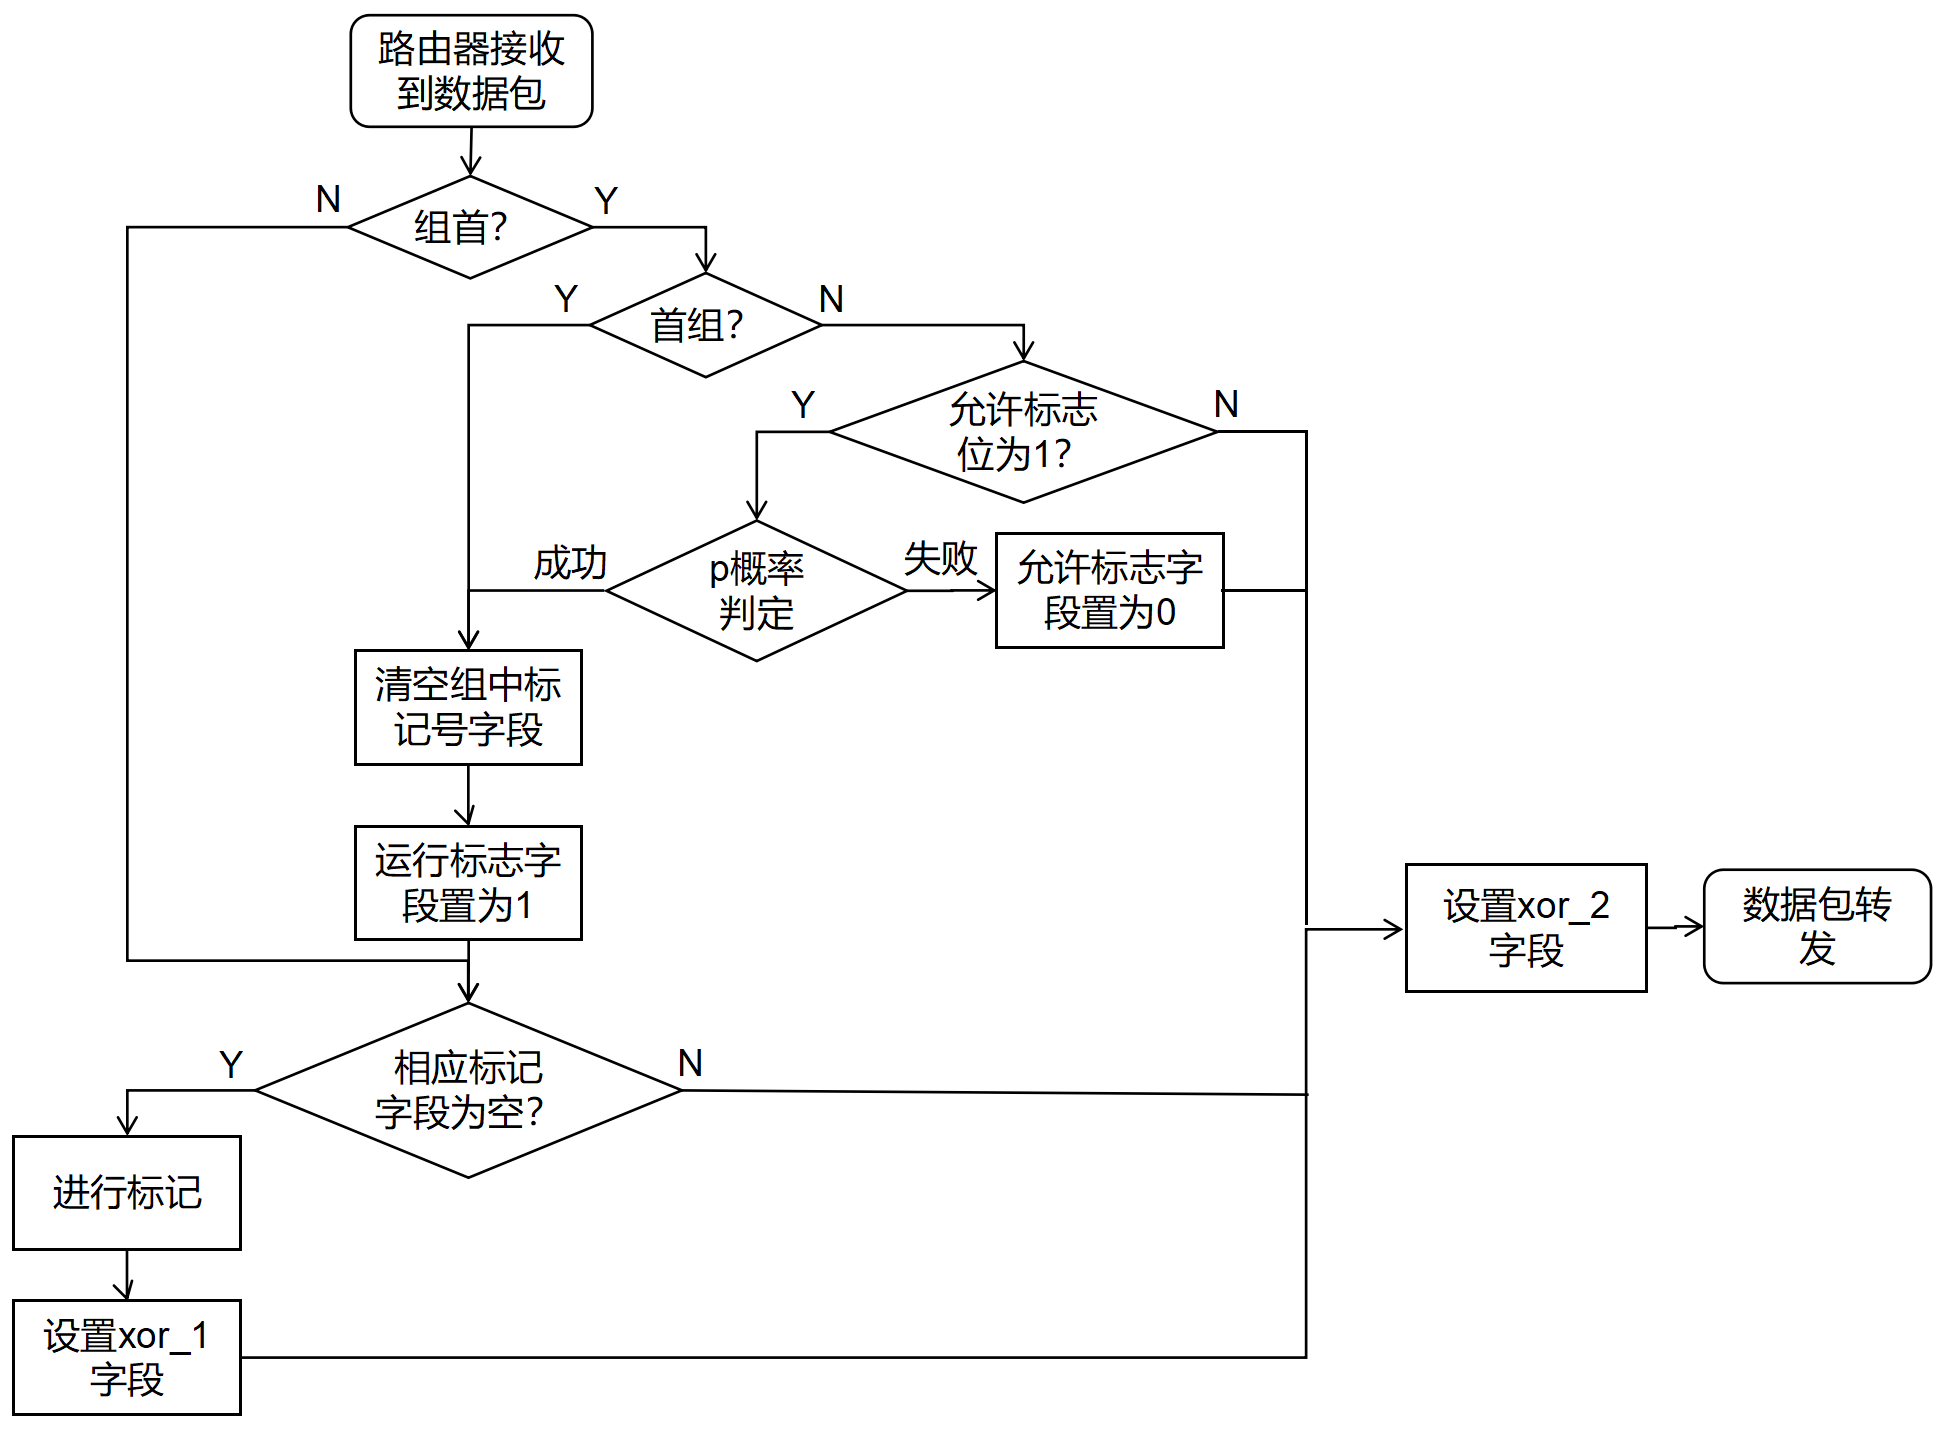
\includegraphics[width = 0.9\textwidth]{marking_procedure.png}
	\caption{路由器标记操作流程图}
	\label{fig:marking_procedure}
\end{figure}
在进行具体的标记操作时,组首路由器会根据先前确定的概率来决定是否对数据包进行标记。\par
若组首路由器决定进行标记,它首先会清空MarkInfo中的所有接口号标记字段(即interface\_i,其中i取值范围为[0,m-1])。
随后,组内的所有路由器将与组首路由器执行相同的操作,检查是否存在空的接口号标记字段。
若存在空字段,则直接将对应的输入接口号填充进去。
若存在空字段,则直接将对应的输入接口号填充进去。
同时,计算xor\_1(如公式\ref{eq:xor1}所示)和xor\_2(如公式\ref{eq:xor2}所示)的值,并将它们分别写入相应的异或字段。\par
\begin{equation}
	\label{eq:xor1}
	xor\_1 = xor\_1 \oplus input\_interface
	\label{eq:xor1}
	xor\_1 = xor\_1 \oplus input\_interface
\end{equation}
\begin{equation}
	\label{eq:xor2}
	xor\_2 = xor\_2 \oplus input\_interface
	\label{eq:xor2}
	xor\_2 = xor\_2 \oplus input\_interface
\end{equation}
如果不存在空的接口号标记字段,表明本组均不对此数据包进行标记,接收到该数据包的路由器也将不会对其进行标记。
在这种情况下,路由器仅计算xor\_2的值,并将其写入xor\_2字段中。\par

另一方面,如果组首路由器基于概率判断决定不对数据包进行标记,它会将allow\_mark字段的值设置为0。
这一操作是为了通知后续的组,不再对该数据包进行概率性的标记操作,以确保标记信息的连续性。\par
这一操作是为了通知后续的组,不再对该数据包进行概率性的标记操作,以确保标记信息的连续性。\par

通过这些操作,当数据包顺利抵达接收者时,其MarkInfo中的interface字段已经记录了一组路由器的输入接口号。
同时,MarkInfo中的xor\_1字段的值将等于所有对数据包进行标记的路由器输入接口号的异或,而xor\_2字段的值则等于路径上所有路由器输入接口号异或。
通过这些操作,当数据包顺利抵达接收者时,其MarkInfo中的interface字段已经记录了一组路由器的输入接口号。
同时,MarkInfo中的xor\_1字段的值将等于所有对数据包进行标记的路由器输入接口号的异或,而xor\_2字段的值则等于路径上所有路由器输入接口号异或。
当接收者接收到一定数量的标记数据包后便可以提取这些信息执行路径重构算法完成路径重构。
\subsection{标记数据包收集阶段}
\subsection{标记数据包收集阶段}
在正常情况下,当服务器未检测到攻击时,系统不会主动进行标记数据包的收集工作,以确保服务器的正常运行和性能不受影响。
然而,一旦服务器检测到遭受攻击的迹象,便会立即启动标记数据包的收集机制,该机制的运行流程如下:\par

1)~初始化路径信息数组\par
收集系统首先会初始化一个本文设计的如图~\ref{fig:markinfo_list}~所示的路径信息结构体数组(PathInfos),用于管理不同待重构的路径信息。
然而,一旦服务器检测到遭受攻击的迹象,便会立即启动标记数据包的收集机制,该机制的运行流程如下:\par

1)~初始化路径信息数组\par
收集系统首先会初始化一个本文设计的如图~\ref{fig:markinfo_list}~所示的路径信息结构体数组(PathInfos),用于管理不同待重构的路径信息。
\begin{figure}[h]
	\centering
	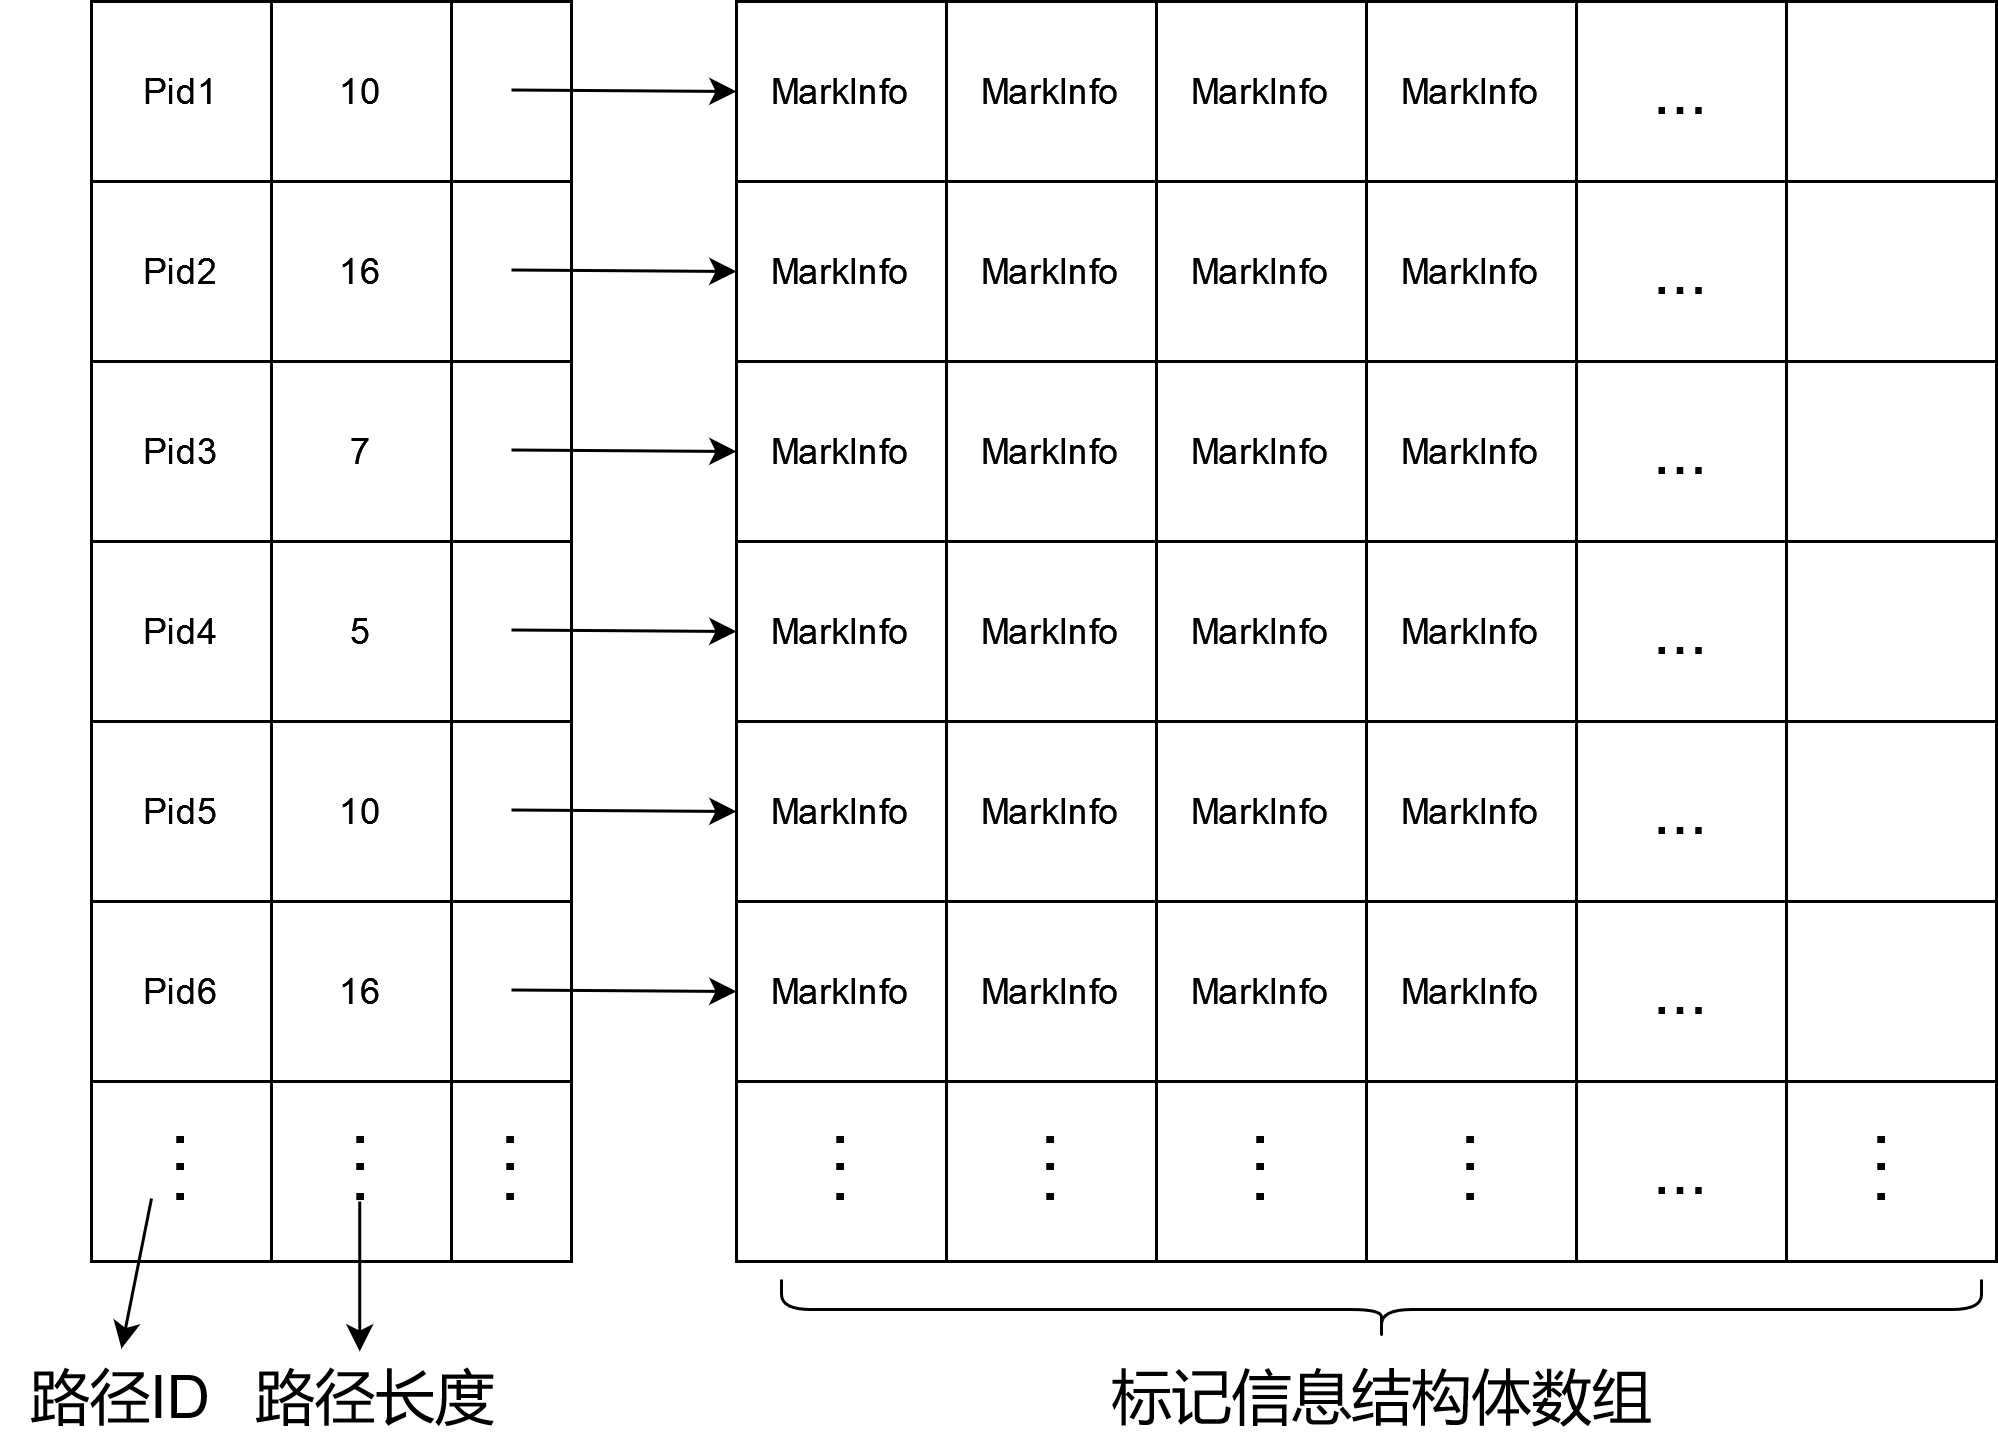
\includegraphics[width = 0.8\textwidth]{mark_list_structure.drawio.png}
	\caption{本文设计的用于管理路径重构信息的数组}
	\label{fig:markinfo_list}
\end{figure}
路径信息结构体包含路径ID(Pid)、路径长度(PLen,由路由器跳数表示)以及指向存放标记信息(MarkInfo)数组的指针。
	\centering
	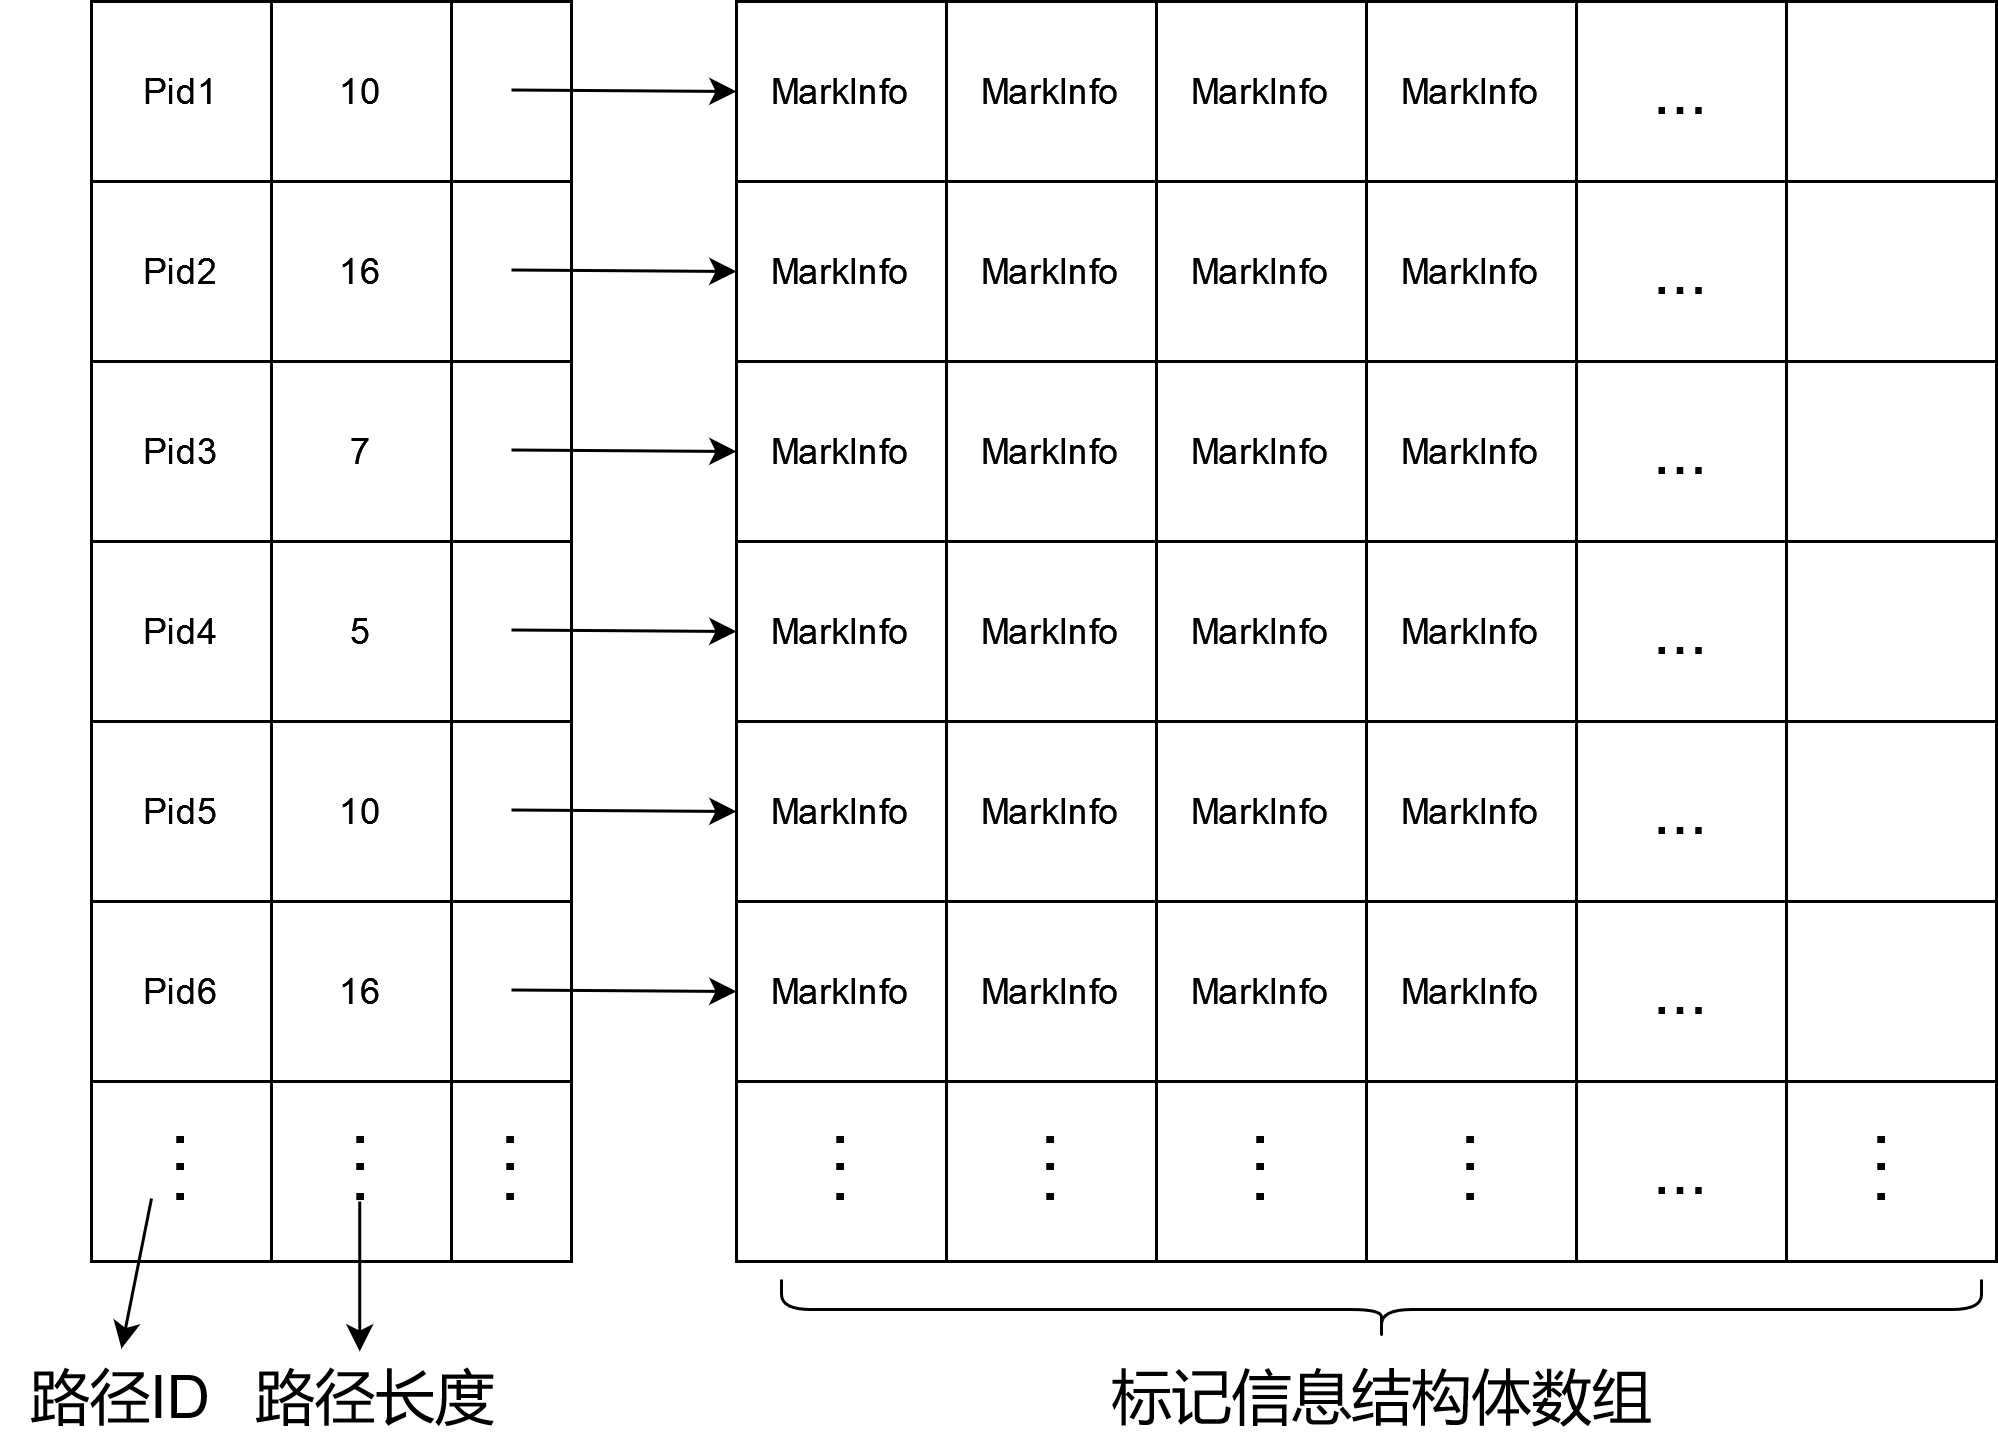
\includegraphics[width = 0.8\textwidth]{mark_list_structure.drawio.png}
	\caption{本文设计的用于管理路径重构信息的数组}
	\label{fig:markinfo_list}
\end{figure}
路径信息结构体包含路径ID(Pid)、路径长度(PLen,由路由器跳数表示)以及指向存放标记信息(MarkInfo)数组的指针。
这样的设计使得系统能够高效地存储和检索路径信息。\par

2)~生成路径编码并查找路径\par
收集系统从网络流量中筛选出与攻击流量相关的数据包,并将数据包中的TTL字段和MarkInfo中的xor\_2字段拼接生成路径编码。
TTL字段指示数据包在网络中的生存时间,而xor\_2字段记录数据包经过的所有路由器输入接口号的异或值。
2)~生成路径编码并查找路径\par
收集系统从网络流量中筛选出与攻击流量相关的数据包,并将数据包中的TTL字段和MarkInfo中的xor\_2字段拼接生成路径编码。
TTL字段指示数据包在网络中的生存时间,而xor\_2字段记录数据包经过的所有路由器输入接口号的异或值。
利用这两个字段的组合,系统能够为每条传输路径生成唯一的编码。
随后,系统利用这个路径编码在PathInfos中查找是否存在相应的路径信息。
如果找到匹配项,进入步骤4);否则,进入步骤3)。\par
如果找到匹配项,进入步骤4);否则,进入步骤3)。\par

3)~初始化新路径信息\par
3)~初始化新路径信息\par
当PathInfos中不存在与当前路径编码匹配的信息时,系统执行以下操作:
\begin{enumerate}[a.]
	\item 确定数据包初始TTL值:数据包初始TTL值根据发送方系统而定,常见值有\{32,64,128,255\}\cite{liu2007dynamic}。 其中大于数据包当前TTL的最小值便为数据包初始TTL值。 
	\item 计算路径长度:将数据包初始TTL与当前TTL相减,得到的差值便是数据包从发送者到接收者所经过的路由器跳数,即路径长度。
	\item 将路径长度和路径编码添加到PathInfos中相应元素的字段中。
	\item 分配内存空间用于存放新路径的标记信息数组,并更新PathInfos中对应元素的指针,使其指向该数组。
	\item 启动一个针对新路径的重组程序,并建立与该路径的发布者订阅者关系。
\begin{enumerate}[a.]
	\item 确定数据包初始TTL值:数据包初始TTL值根据发送方系统而定,常见值有\{32,64,128,255\}\cite{liu2007dynamic}。 其中大于数据包当前TTL的最小值便为数据包初始TTL值。 
	\item 计算路径长度:将数据包初始TTL与当前TTL相减,得到的差值便是数据包从发送者到接收者所经过的路由器跳数,即路径长度。
	\item 将路径长度和路径编码添加到PathInfos中相应元素的字段中。
	\item 分配内存空间用于存放新路径的标记信息数组,并更新PathInfos中对应元素的指针,使其指向该数组。
	\item 启动一个针对新路径的重组程序,并建立与该路径的发布者订阅者关系。
\end{enumerate}
\par

4)~写入标记信息并通知重组程序\par
执行完步骤3)~后,PathInfos中已经存在与当前路径编码匹配的信息,此时执行以下操作:
\begin{enumerate}[a.]
	\item 从当前操作的攻击数据包中提取MarkInfo。
	\item 将提取的MarkInfo追加到对应路径的标记信息数组中。
	\item 通知在该路径上进行订阅的重组程序进行处理。
4)~写入标记信息并通知重组程序\par
执行完步骤3)~后,PathInfos中已经存在与当前路径编码匹配的信息,此时执行以下操作:
\begin{enumerate}[a.]
	\item 从当前操作的攻击数据包中提取MarkInfo。
	\item 将提取的MarkInfo追加到对应路径的标记信息数组中。
	\item 通知在该路径上进行订阅的重组程序进行处理。
\end{enumerate}
\par
5)~重复执行直至停止溯源\par
从第步骤2)~到步骤4)~的操作将重复执行,直到系统接收到停止溯源的指令或网络流量中不再出现与攻击相关的数据包为止。\par
5)~重复执行直至停止溯源\par
从第步骤2)~到步骤4)~的操作将重复执行,直到系统接收到停止溯源的指令或网络流量中不再出现与攻击相关的数据包为止。\par

通过这些操作的循环执行,收集系统能够实现对网络流量的持续监控,确保及时捕获与攻击相关的数据包。
同时,系统也能够及时通知路径重构程序进行实时溯源,从而高效处理海量网络数据。

\subsection{路径重组阶段}
一旦PathInfos中出现相应的路径信息,该路径对应的路径重组程序便被创建。

\subsection{路径重组阶段}
一旦PathInfos中出现相应的路径信息,该路径对应的路径重组程序便被创建。
路径重组程序的流程如下:\par
1)~初始化变量:\par
\begin{enumerate}[a.]
	\item 创建一个cur\_xor变量,初始值设为对应标记信息结构体中的xor\_2。该变量将作为路径重构的关键线索。
	\item 创建一个cur\_len变量,初始值设为0。用于记录当前路径重构的长度。
	\item 初始化一个路径重构队列path\_queue,用于存储重构过程中得到的接口号序列。
1)~初始化变量:\par
\begin{enumerate}[a.]
	\item 创建一个cur\_xor变量,初始值设为对应标记信息结构体中的xor\_2。该变量将作为路径重构的关键线索。
	\item 创建一个cur\_len变量,初始值设为0。用于记录当前路径重构的长度。
	\item 初始化一个路径重构队列path\_queue,用于存储重构过程中得到的接口号序列。
\end{enumerate}

2)~查找匹配的MarkInfo:\par
\begin{enumerate}[a.]
	\item 从对应的MarkInfo数组中查找是否存在MarkInfo.xor\_1与cur\_xor相等的记录。
	\item 如果找到匹配项,进入步骤4);否则,进入步骤3)。
2)~查找匹配的MarkInfo:\par
\begin{enumerate}[a.]
	\item 从对应的MarkInfo数组中查找是否存在MarkInfo.xor\_1与cur\_xor相等的记录。
	\item 如果找到匹配项,进入步骤4);否则,进入步骤3)。
\end{enumerate}

3)~等待新数据:\par
\begin{enumerate}[a.]
	\item 将当前重组程序置为阻塞状态,等待收集系统发布新的MarkInfo数据。
	\item 当接收到新数据时,判断其MarkInfo.xor\_1是否与cur\_xor相等。
	\item 如果相等,进入步骤4);否则,继续阻塞并等待新数据。
3)~等待新数据:\par
\begin{enumerate}[a.]
	\item 将当前重组程序置为阻塞状态,等待收集系统发布新的MarkInfo数据。
	\item 当接收到新数据时,判断其MarkInfo.xor\_1是否与cur\_xor相等。
	\item 如果相等,进入步骤4);否则,继续阻塞并等待新数据。
\end{enumerate}

4)~更新路径重构信息:\par
\begin{enumerate}[a.]
	\item 将找到的MarkInfo中的interface\_i逆序放入path\_queue中。
	\item 根据公式重新计算cur\_xor的值,计算方式如公式~\ref{eq:calculateXor}~所示。
	      \begin{equation}
		      \label{eq:calculateXor}
		      cur\_xor = cur\_xor \oplus interface\_1 \oplus interface\_2 \oplus \cdots \oplus interface\_m
	      \end{equation}
	\item 更新cur\_len的值:cur\_len = cur\_len + m。
4)~更新路径重构信息:\par
\begin{enumerate}[a.]
	\item 将找到的MarkInfo中的interface\_i逆序放入path\_queue中。
	\item 根据公式重新计算cur\_xor的值,计算方式如公式~\ref{eq:calculateXor}~所示。
	      \begin{equation}
		      \label{eq:calculateXor}
		      cur\_xor = cur\_xor \oplus interface\_1 \oplus interface\_2 \oplus \cdots \oplus interface\_m
	      \end{equation}
	\item 更新cur\_len的值:cur\_len = cur\_len + m。
\end{enumerate}

5)~判断路径重构状态:\par
\begin{enumerate}[a.]
	\item 比较cur\_len与PLen的值。
	\item 如果cur\_len等于PLen,进一步检查cur\_xor是否等于0。
	\item 如果cur\_xor不等于0,表明构建失败,进入步骤6)。
	\item 如果cur\_xor等于0,表明构建成功,进入步骤7)。
	\item 如果cur\_len不等于PLen,表明路径重构尚未完成,返回步骤2)~并按照当前的路径重构状态继续匹配MarkInfo完成重构。
5)~判断路径重构状态:\par
\begin{enumerate}[a.]
	\item 比较cur\_len与PLen的值。
	\item 如果cur\_len等于PLen,进一步检查cur\_xor是否等于0。
	\item 如果cur\_xor不等于0,表明构建失败,进入步骤6)。
	\item 如果cur\_xor等于0,表明构建成功,进入步骤7)。
	\item 如果cur\_len不等于PLen,表明路径重构尚未完成,返回步骤2)~并按照当前的路径重构状态继续匹配MarkInfo完成重构。
\end{enumerate}


6)~处理构建失败情况:\par
6)~处理构建失败情况:\par
如果路径构建失败,可能是由于数据不完整或路径信息错误。
此时,可以根据实际情况选择重新收集数据或标记该路径为无效。\par

7)~返回重构结果:\par
\begin{enumerate}[a.]
	\item 将距离受害者服务器最近的路由器作为当前路由器,利用path\_queue中存储的第一个接口号在当前路由器中进行查找是否存在对应的路由器。
	\item 如果成功找到与当前接口号匹配的路由器,则将其设定为当前路由器。
	\item 继续按照接口号序列中的下一个接口号进行查找。
	\item 以上操作重复执行,如果在查找过程中发现当前路由器不存在接口号序列中待查找的接口号,即查找失败,说明路径重构结果错误。
	\item 当接口号序列中的最后一个接口号成功匹配到相应的路由器时,说明路径重构结果正确。找到的最后一个路由器即为攻击者的最近邻路由器。
\end{enumerate}

\subsection{溯源速度实验评估}
7)~返回重构结果:\par
\begin{enumerate}[a.]
	\item 将距离受害者服务器最近的路由器作为当前路由器,利用path\_queue中存储的第一个接口号在当前路由器中进行查找是否存在对应的路由器。
	\item 如果成功找到与当前接口号匹配的路由器,则将其设定为当前路由器。
	\item 继续按照接口号序列中的下一个接口号进行查找。
	\item 以上操作重复执行,如果在查找过程中发现当前路由器不存在接口号序列中待查找的接口号,即查找失败,说明路径重构结果错误。
	\item 当接口号序列中的最后一个接口号成功匹配到相应的路由器时,说明路径重构结果正确。找到的最后一个路由器即为攻击者的最近邻路由器。
\end{enumerate}

\subsection{溯源速度实验评估}
\textbf{1.数据集介绍}\par
CAIDA IPv4 Prefix-Probing Traceroute Dataset是CAIDA机构精心设计的大型网络数据集,它通过主动测量技术,利用全球范围内的测量点向特定的IPv4前缀发送Traceroute请求,并详细记录响应结果。
这一数据集涵盖了20,377,233条路径追踪记录,涉及899,916个不同的IP地址,深入揭示了互联网的拓扑结构和动态行为。
为了研究的准确性,本文仅采用了那些能够成功到达指定目的地且没有循环的部分路径追踪记录。
\par
CAIDA IPv4 Prefix-Probing Traceroute Dataset是CAIDA机构精心设计的大型网络数据集,它通过主动测量技术,利用全球范围内的测量点向特定的IPv4前缀发送Traceroute请求,并详细记录响应结果。
这一数据集涵盖了20,377,233条路径追踪记录,涉及899,916个不同的IP地址,深入揭示了互联网的拓扑结构和动态行为。
为了研究的准确性,本文仅采用了那些能够成功到达指定目的地且没有循环的部分路径追踪记录。
\par
\textbf{2.实验评估指标}\par
在本次溯源速度测试中,本文使用完成路径重构所需收集的数据包数量作为关键验证指标。
在本次溯源速度测试中,本文使用完成路径重构所需收集的数据包数量作为关键验证指标。
数据包数量是衡量溯源速度的重要指标之一,因为它直接关系到网络路径回溯或安全分析任务的执行效率和速度。
通过减少完成溯源所需的数据包数量,可以显著提升溯源的速度,从而更快地获取分析结果。
这不仅能够减少网络负载,降低资源消耗,还能提高整体分析效率,为网络安全的实时监测和响应提供有力支持。
因此,在本次实验中,本文重点验证了本方案在减少数据包数量方面的优势。\par
因此,在本次实验中,本文重点验证了本方案在减少数据包数量方面的优势。\par

\textbf{3.实验设计}\par
本文从数据集中筛选出跳数达到最大的追踪记录,并将这些记录中的目的结点作为受害者结点。
随后,本文按照距离d从1开始递增的方式,随机选取距离受害者d跳的结点,模拟攻击结点向向受害者结点发送攻击数据包。
随后,本文按照距离d从1开始递增的方式,随机选取距离受害者d跳的结点,模拟攻击结点向向受害者结点发送攻击数据包。
受害者结点负责收集这些数据包,并应用路径重构算法来还原数据包的传输路径。
为了确保实验结果的可靠性和一致性,本文对每个距离d都进行了1,000次重复实验并取平均值。
此外,为了模拟更真实的实验环境,本文还引入了一些额外的结点作为用户结点。
为了确保实验结果的可靠性和一致性,本文对每个距离d都进行了1,000次重复实验并取平均值。
此外,为了模拟更真实的实验环境,本文还引入了一些额外的结点作为用户结点。
这些用户结点模拟了实际网络中的其他用户活动,增加了实验的复杂性和真实性。\par

\textbf{4.实验结果与分析}\par
图\ref{fig:packets_num}是本方案在m=2和m=4的情况下,与PPM-Fixed\cite{Zhou2019Linna}和PPM-Dynamic方案\cite{liu2007dynamic}相比,完成不同距离的路由回溯所需的最少数据包数量与路径长度之间的关系。
\begin{figure}[htbp]
	\centering
	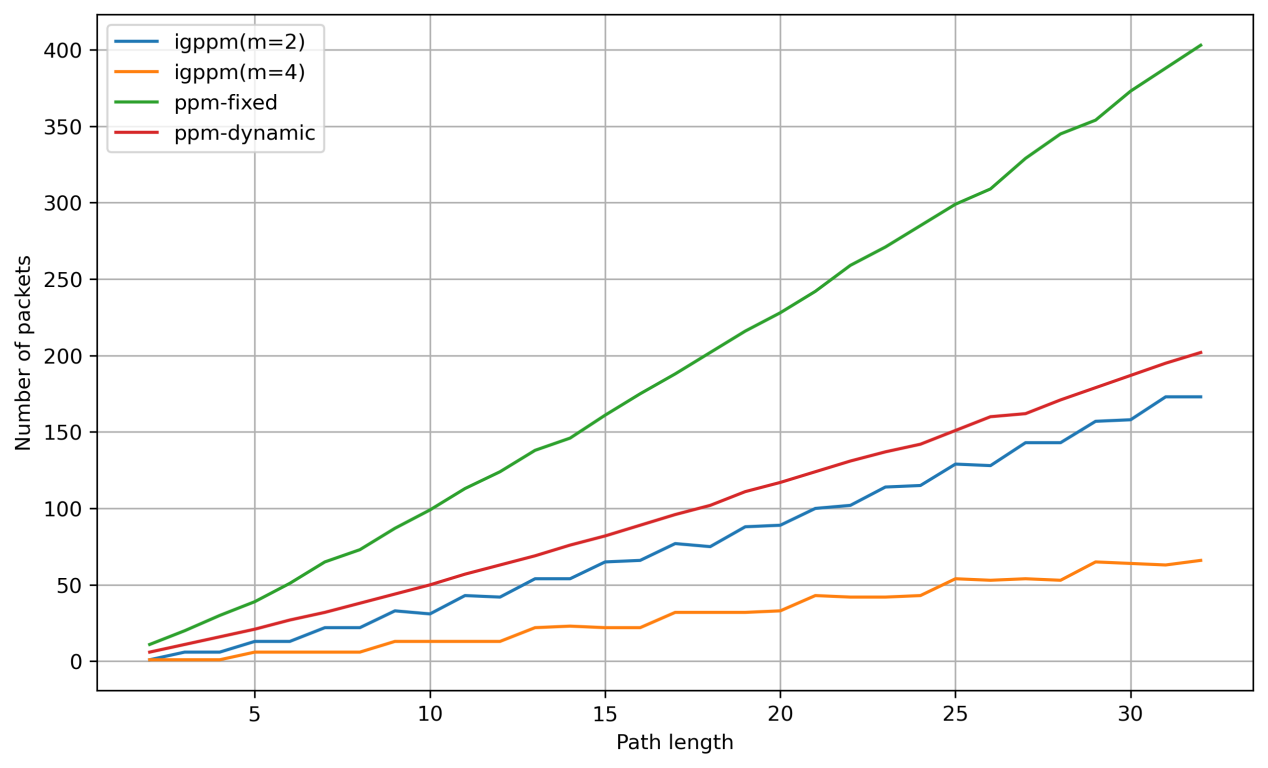
\includegraphics[width = 0.8\textwidth]{packets_num.png}
	\caption{路径重建所需数据包数量与路径长度关系}
	\label{fig:packets_num}
\end{figure}
	\centering
	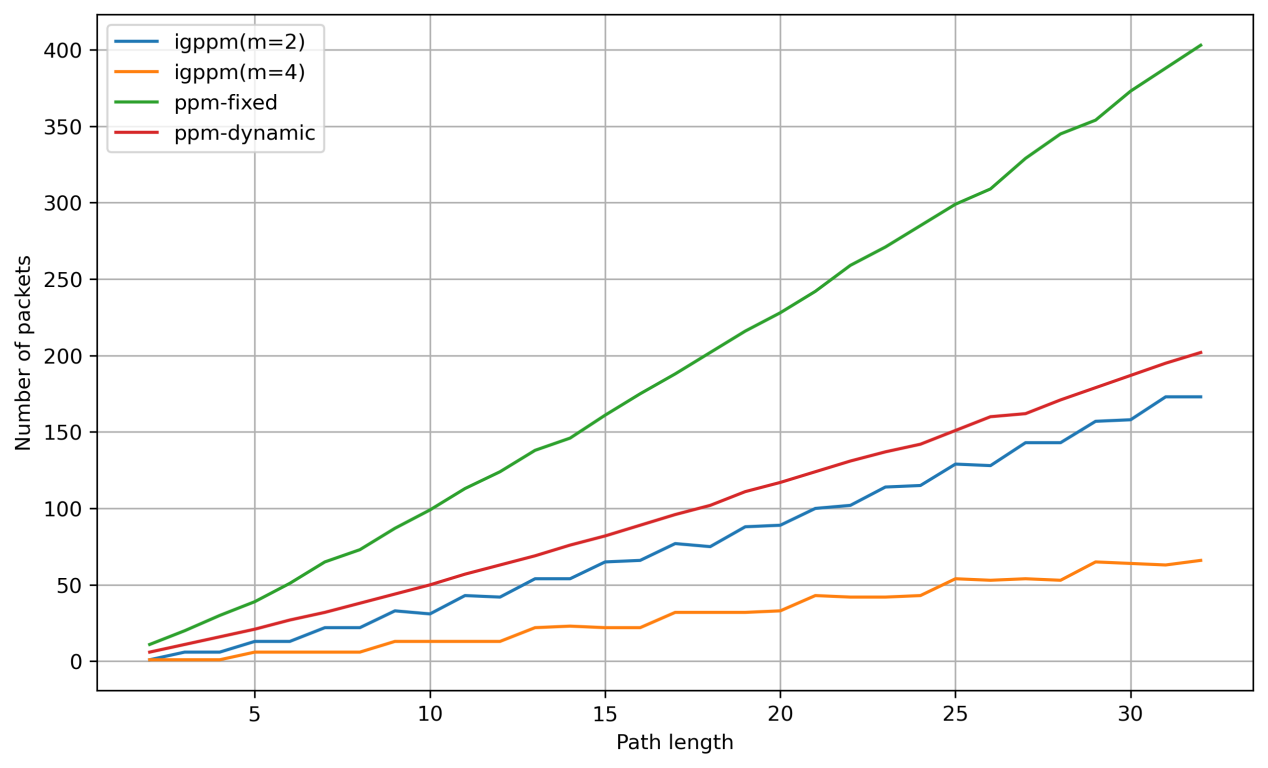
\includegraphics[width = 0.8\textwidth]{packets_num.png}
	\caption{路径重建所需数据包数量与路径长度关系}
	\label{fig:packets_num}
\end{figure}
从图中可以看出,本文提出的方案在完成路径重构时所需要的数据包数量要远远少于PPM-Fixed方案。
当m=2时,本方案略优于PPM-Dynamic方案;当m=4时,则明显优于以上两种PPM类方案。
这一结果表明,本方案在溯源速度方面具有显著优势。
此外,仔细观察图像可以发现,本文提出的方案表现出阶梯性特征。
这是因为该方案采用了分组标记的策略:无论跳数d相差多少,只要$k=\lceil d/m \rceil$相同,完成路径重构所需要的数据包数量就会相同。\par
这是因为该方案采用了分组标记的策略:无论跳数d相差多少,只要$k=\lceil d/m \rceil$相同,完成路径重构所需要的数据包数量就会相同。\par

通过以上的实验验证和结果分析,本方案相较于传统的PPM方案,在溯源速度方面展现出了明显的优越性。
通过以上的实验验证和结果分析,本方案相较于传统的PPM方案,在溯源速度方面展现出了明显的优越性。
另外值得注意的是,在传统的PPM类方案中,路径重构所需的数据包数量通常指的是实现路由覆盖所需的最少数据包数量。
因此,在本文中,对于PPM完成路径重构所需的数据包数量的评估,实际上仅是基于路径覆盖测试的数据包统计。
实际上,如果期望通过数据包的数量关系直接获取一条完整的网络路径,那么所需的数据包数量将会非常庞大。
不过,本文所提方案在完成路径重构时,采用了接口号以及两个异或字段以及TTL来实现溯源,这使得本文的方法在路径重构时具有更高的灵活性和效率。
因此,在本文的方案中,完成路径重构所需的数据包数量即为取得一条实际路径所需的数据包数量,这大大减少了重构路径所需的数据包开销。
\subsection{溯源准确率实验评估}
\subsection{溯源准确率实验评估}
\textbf{1.仿真软件介绍}\par
在本次实验中本文使用NS-3网络模拟器来构建实验环境。
NS-3是一个先进的开源网络模拟器,广泛应用于网络研究和教育领域,它通过离散事件模拟技术支持各种有线、无线网络协议和设备的性能评估。
该模拟器以其模块化设计和丰富的模型库而闻名,允许用户灵活构建复杂的网络场景。\par
\textbf{2.实验设计}\par
本文首先借助NS-3仿真工具构建了一个如图~\ref{fig:network_enviroment}~所示的逻辑拓扑网络,其中包含14个转发结点($R_i$,其中i的范围是1到14),10个作为攻击者结点的数据发送结点($PC_j$,其中j的范围是1到10),以及一个作为受害者结点的数据接收结点(Server)。
\begin{figure}[h]
	\centering
	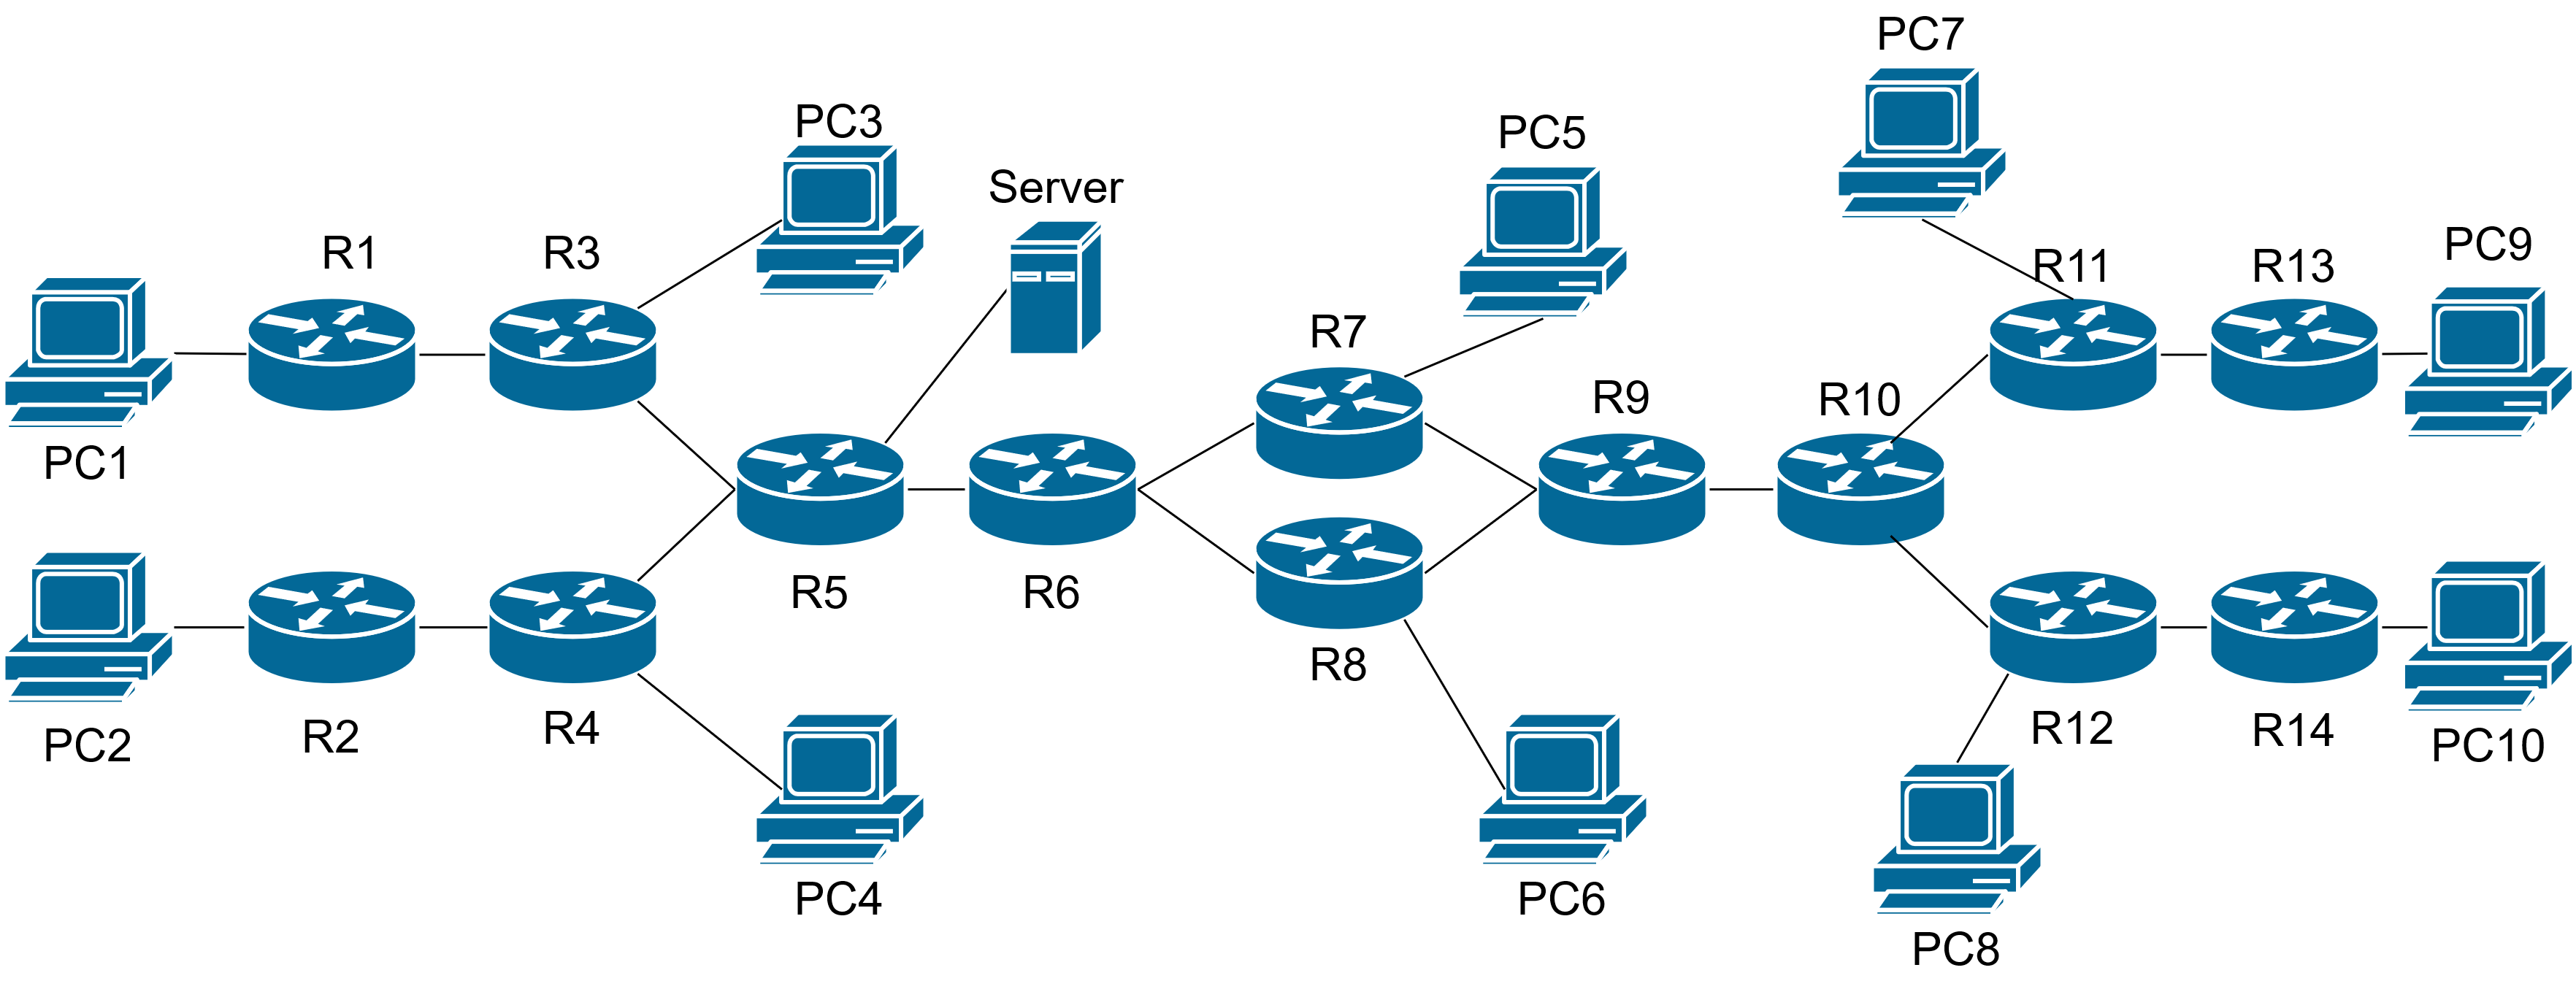
\includegraphics[width=0.8\textwidth]{network_enviroment.drawio.png}
	\caption{NS-3模拟器生成的逻辑拓扑结构}
	\label{fig:network_enviroment}
	\centering
	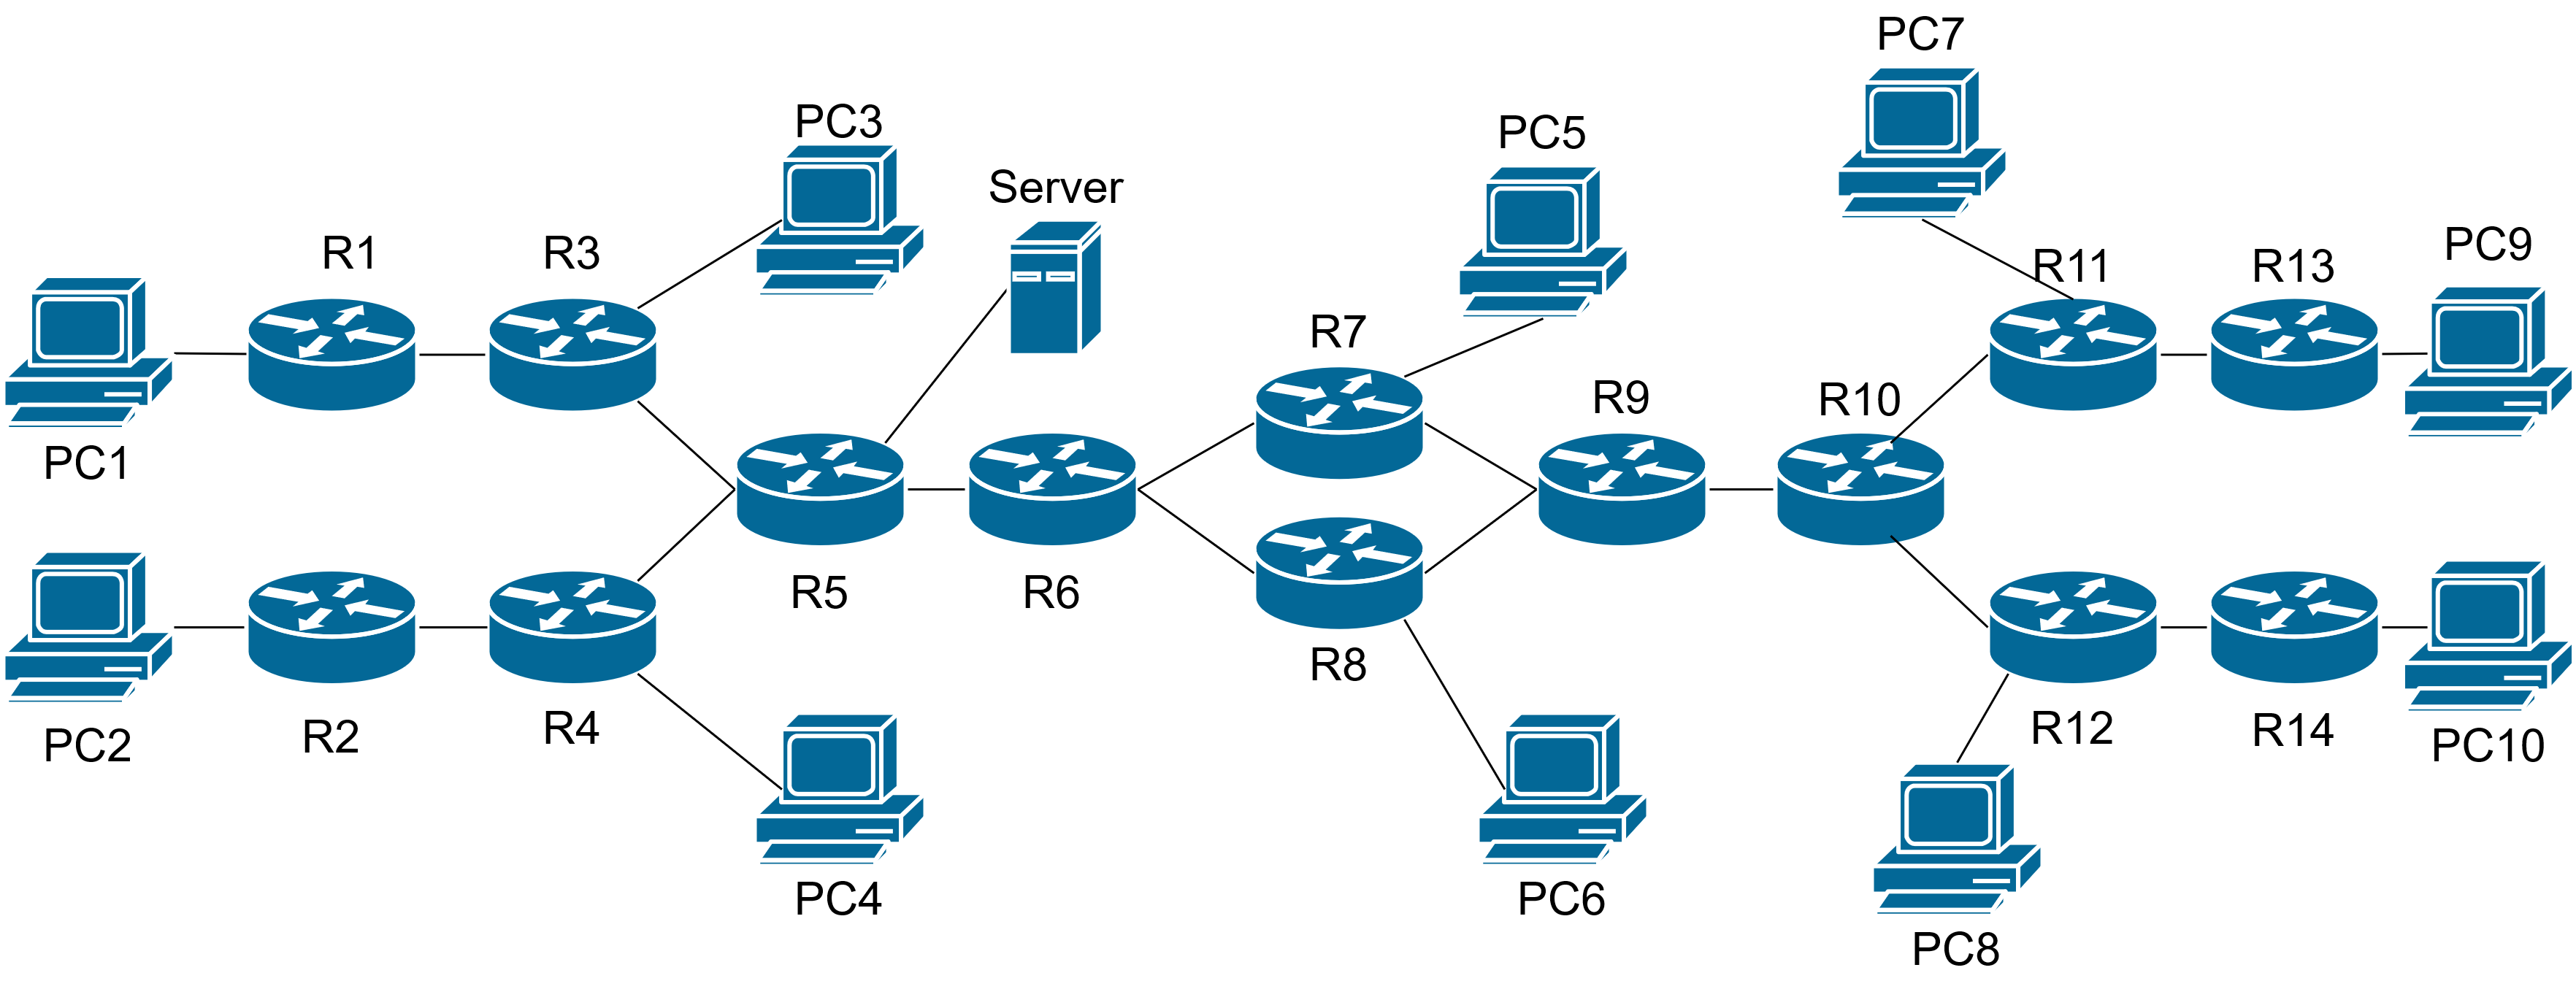
\includegraphics[width=0.8\textwidth]{network_enviroment.drawio.png}
	\caption{NS-3模拟器生成的逻辑拓扑结构}
	\label{fig:network_enviroment}
\end{figure}
为了评估网络在不同攻击规模下的性能表现,本文首先使用5个攻击结点向受害者结点发送攻击数据包。
随后,本文逐步增加攻击结点的数量,以模拟网络遭受更大规模攻击的场景。
当攻击结点数量超过10个时,本文采取了以$R_5$为网络拓扑中心随机添加转发结点的策略,并在每个新添加的转发结点上挂载一个攻击结点,以模拟攻击行为的进一步扩散和复杂化。
为了评估网络在不同攻击规模下的性能表现,本文首先使用5个攻击结点向受害者结点发送攻击数据包。
随后,本文逐步增加攻击结点的数量,以模拟网络遭受更大规模攻击的场景。
当攻击结点数量超过10个时,本文采取了以$R_5$为网络拓扑中心随机添加转发结点的策略,并在每个新添加的转发结点上挂载一个攻击结点,以模拟攻击行为的进一步扩散和复杂化。
以下是本次实验的结果与分析部分。\par
\textbf{3.实验结果与分析}\par
图~\ref{fig:traceback_accuracy}~是本文方案与ICMP Ping方案以及PPM方案在网络仿真环境下的对比结果。
图~\ref{fig:traceback_accuracy}~是本文方案与ICMP Ping方案以及PPM方案在网络仿真环境下的对比结果。
\begin{figure}[h]
	\centering
	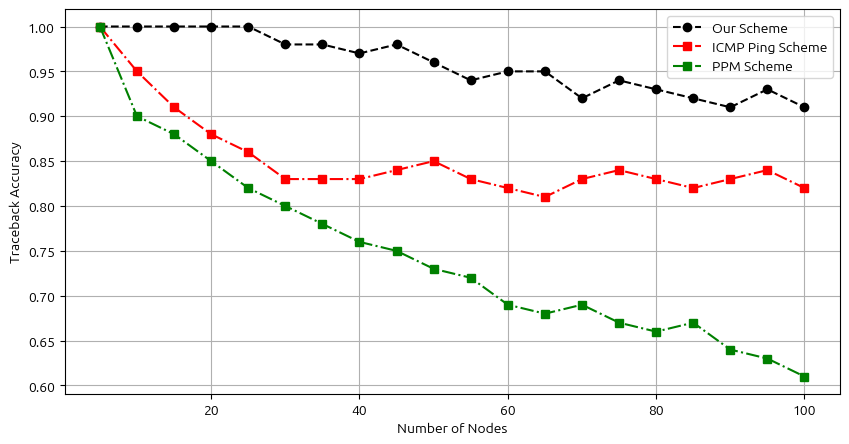
\includegraphics[width=0.8\textwidth]{traceback_accuracy.png}
	\caption{拓扑还原准确率}
	\label{fig:traceback_accuracy}
	\centering
	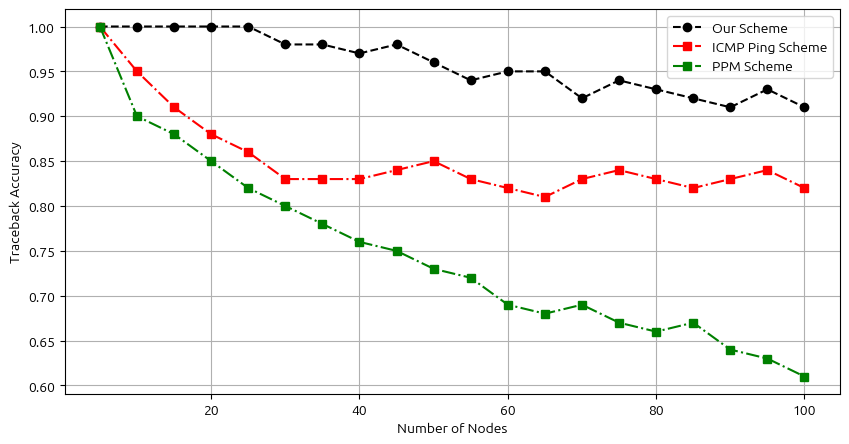
\includegraphics[width=0.8\textwidth]{traceback_accuracy.png}
	\caption{拓扑还原准确率}
	\label{fig:traceback_accuracy}
\end{figure}

从图中可以看出,随着攻击结点数的不断增加,本文的所提出的方案准确率相对较高并且相对稳定。
而ICMP Ping方案以及PPM方案随着结点数的增加,溯源准确率极速下降。
因此可以得出结论,本文所提出的方案相比PPM方案以及ICMP Ping在面对大规模的网络攻击时具有更高的溯源准确率。

\section{基于溯源的模型防护方法}
\subsection{方法设计}
上文已详细阐述了基于路由器接口号成组标记溯源方法的具体内容,并通过实验验证了其在溯源方面的表现效果。
接下来,本文将在此基础上设计检测模型的防护方法。\par
图~\ref{fig:defend_procedure}~是该方法的具体操作流程。
\begin{figure}[h]
	\centering
	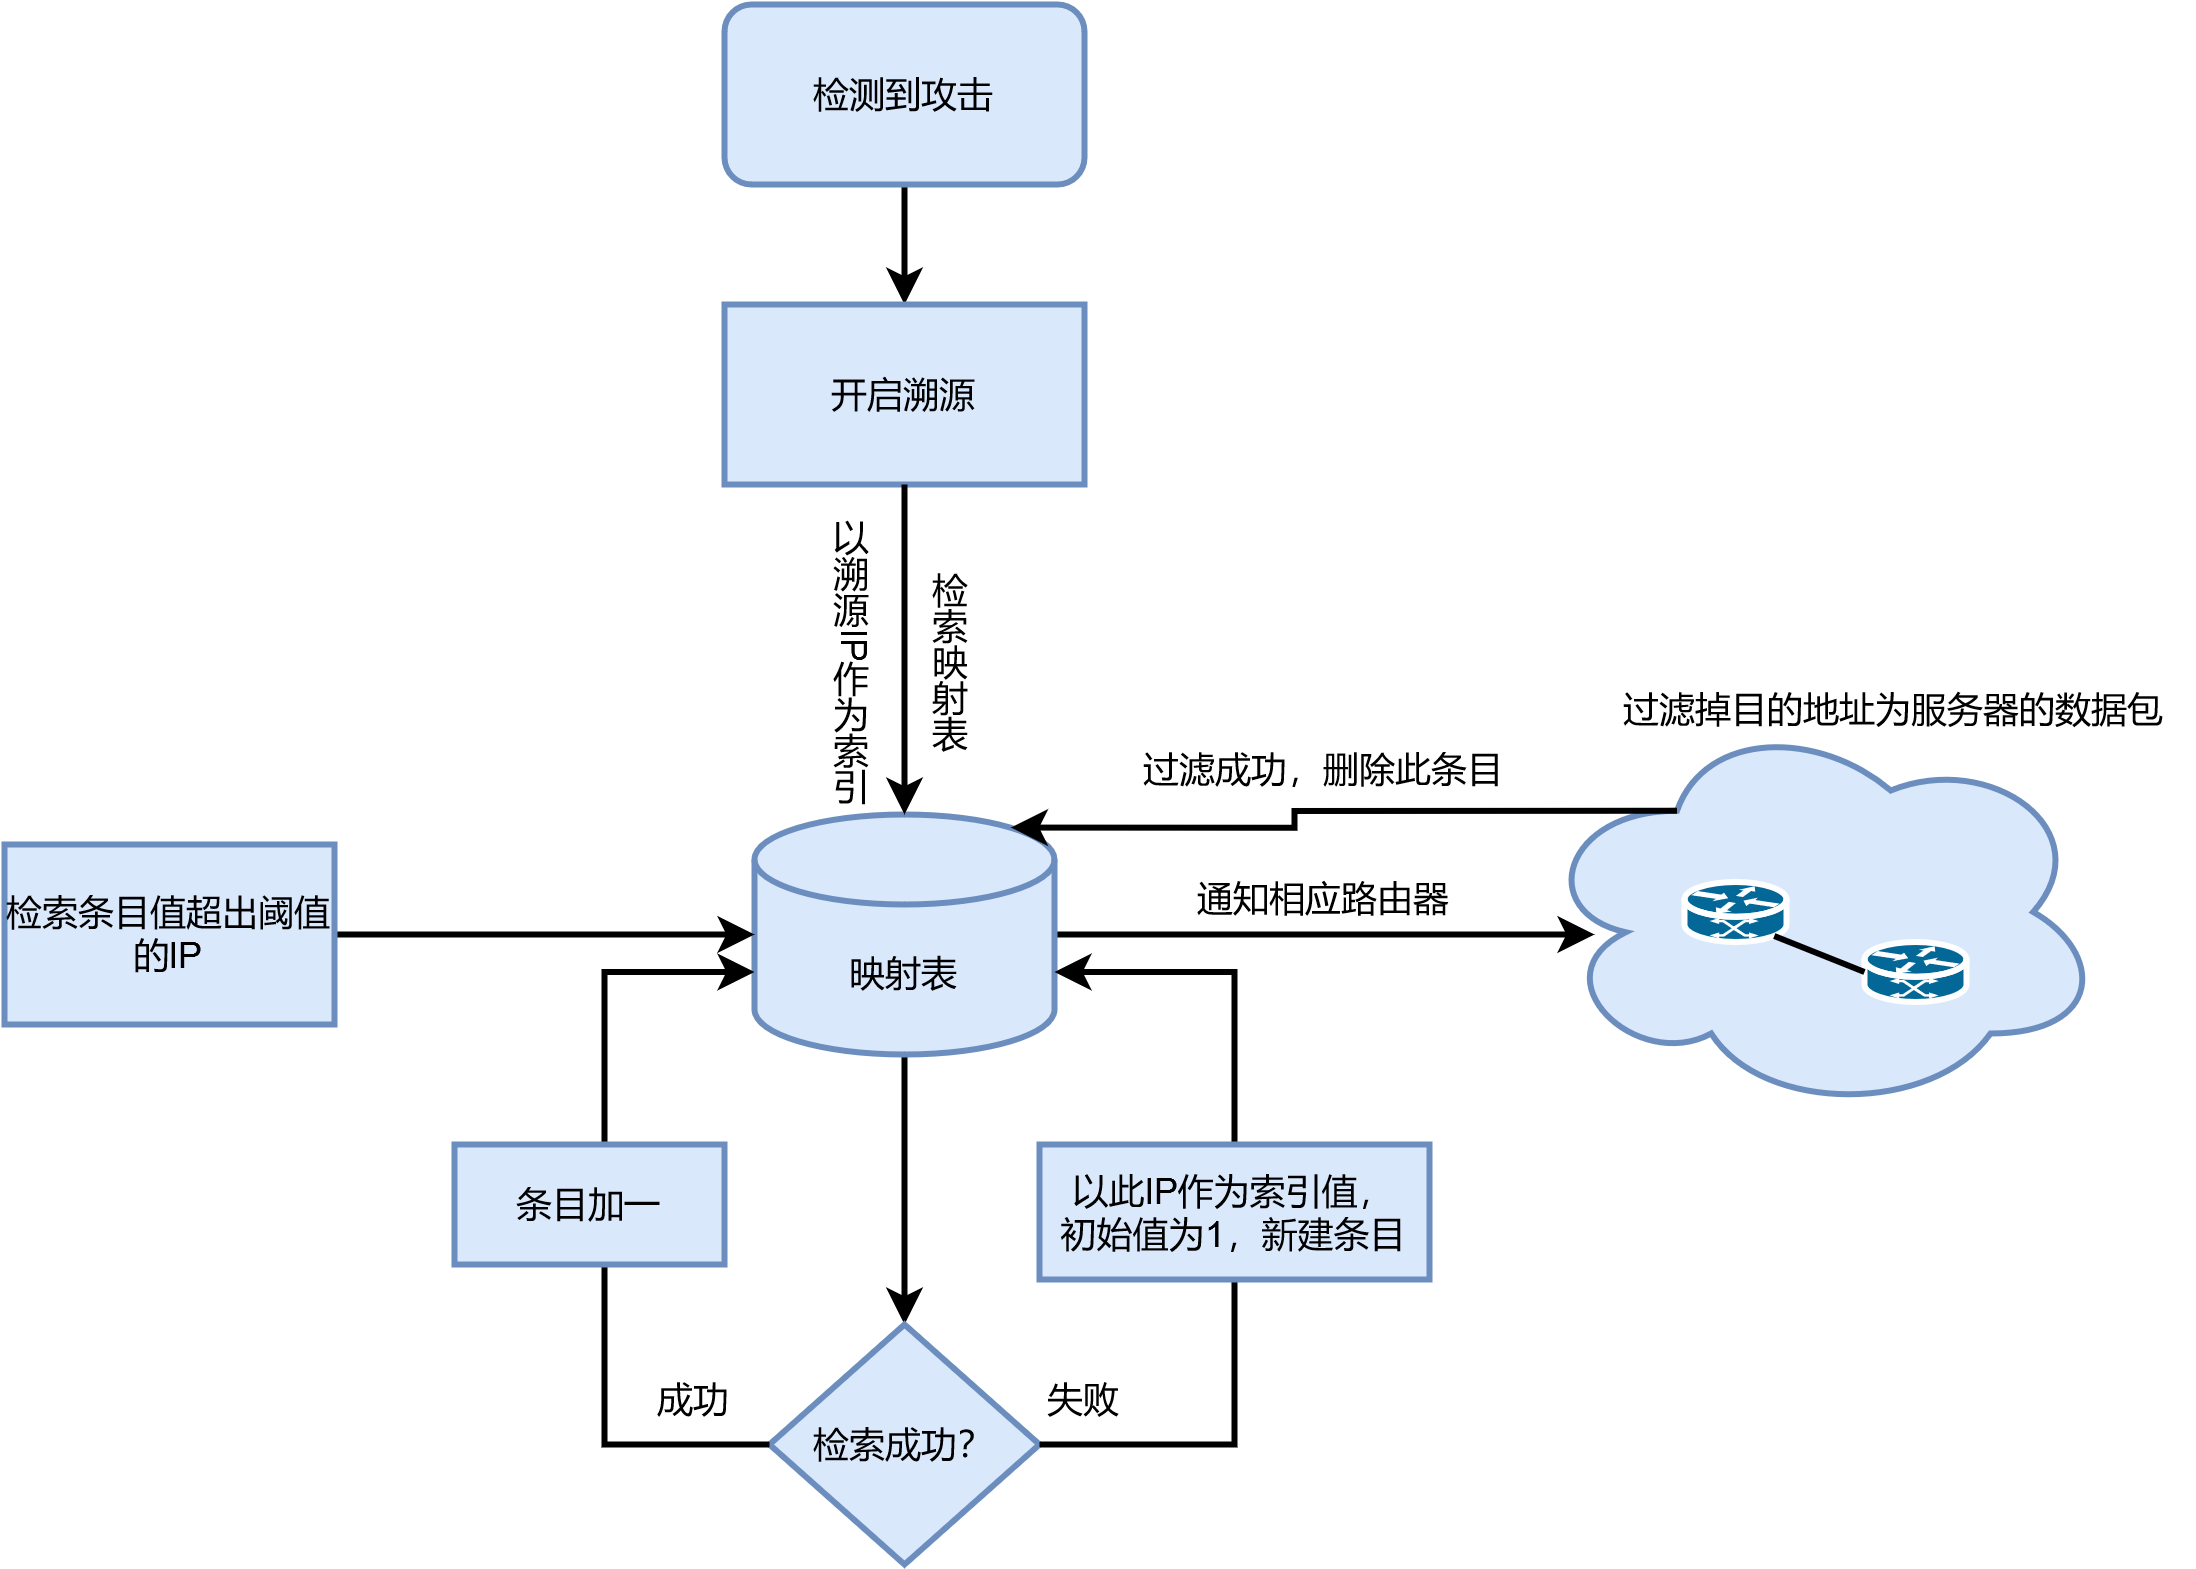
\includegraphics[width=\textwidth]{defend_method.drawio.png}
	\caption{防护流程}
	\label{fig:defend_procedure}
\end{figure}
首先,当检测模型成功检测到攻击流量后,会立即启动溯源机制进行溯源取得溯源结果。
随后,利用溯源结果——即攻击者最近邻的路由器IP作为索引,在映射表中检索对应条目。
其中,映射表是一个用于存储路由器IP地址与对应标记次数之间映射关系的键值对数组。
在这个数组中,IP地址以字符串形式作为索引或键,而与之对应的标记次数则以整数形式作为值。
若在映射表中能够检索到对应条目,则对该条目值进行累加,以实时追踪攻击次数的增长。
若在映射表中不能检索到对应条目,则立即新建一条记录,将溯源获取的IP地址设为索引,并初始化其值为1,为后续累加操作做好准备。
最后,定期检查映射表中是否存在条目值超过预设阈值的情况。
一旦发现有条目值超过阈值,立即通知相关路由器过滤掉发送到该服务器的流量,从而大幅减轻攻击源对检测模型的负担,确保服务器的安全稳定运行。


\subsection{实验评估与分析}
\textbf{1.实验设计}\par
为验证本防护方法的有效性,本文利用VMWare WorkStation构建了一个高度仿真的网络攻击环境,以模拟真实世界中可能遭遇的网络威胁。
图~\ref{fig:vmwarelist}~展示了在VMWare中部署的全部虚拟机列表,所有虚拟机均使用VMnet2网络适配器,确保它们处于同一网络中,从而能够模拟出真实的网络环境。
\begin{figure}[h]
	\centering
	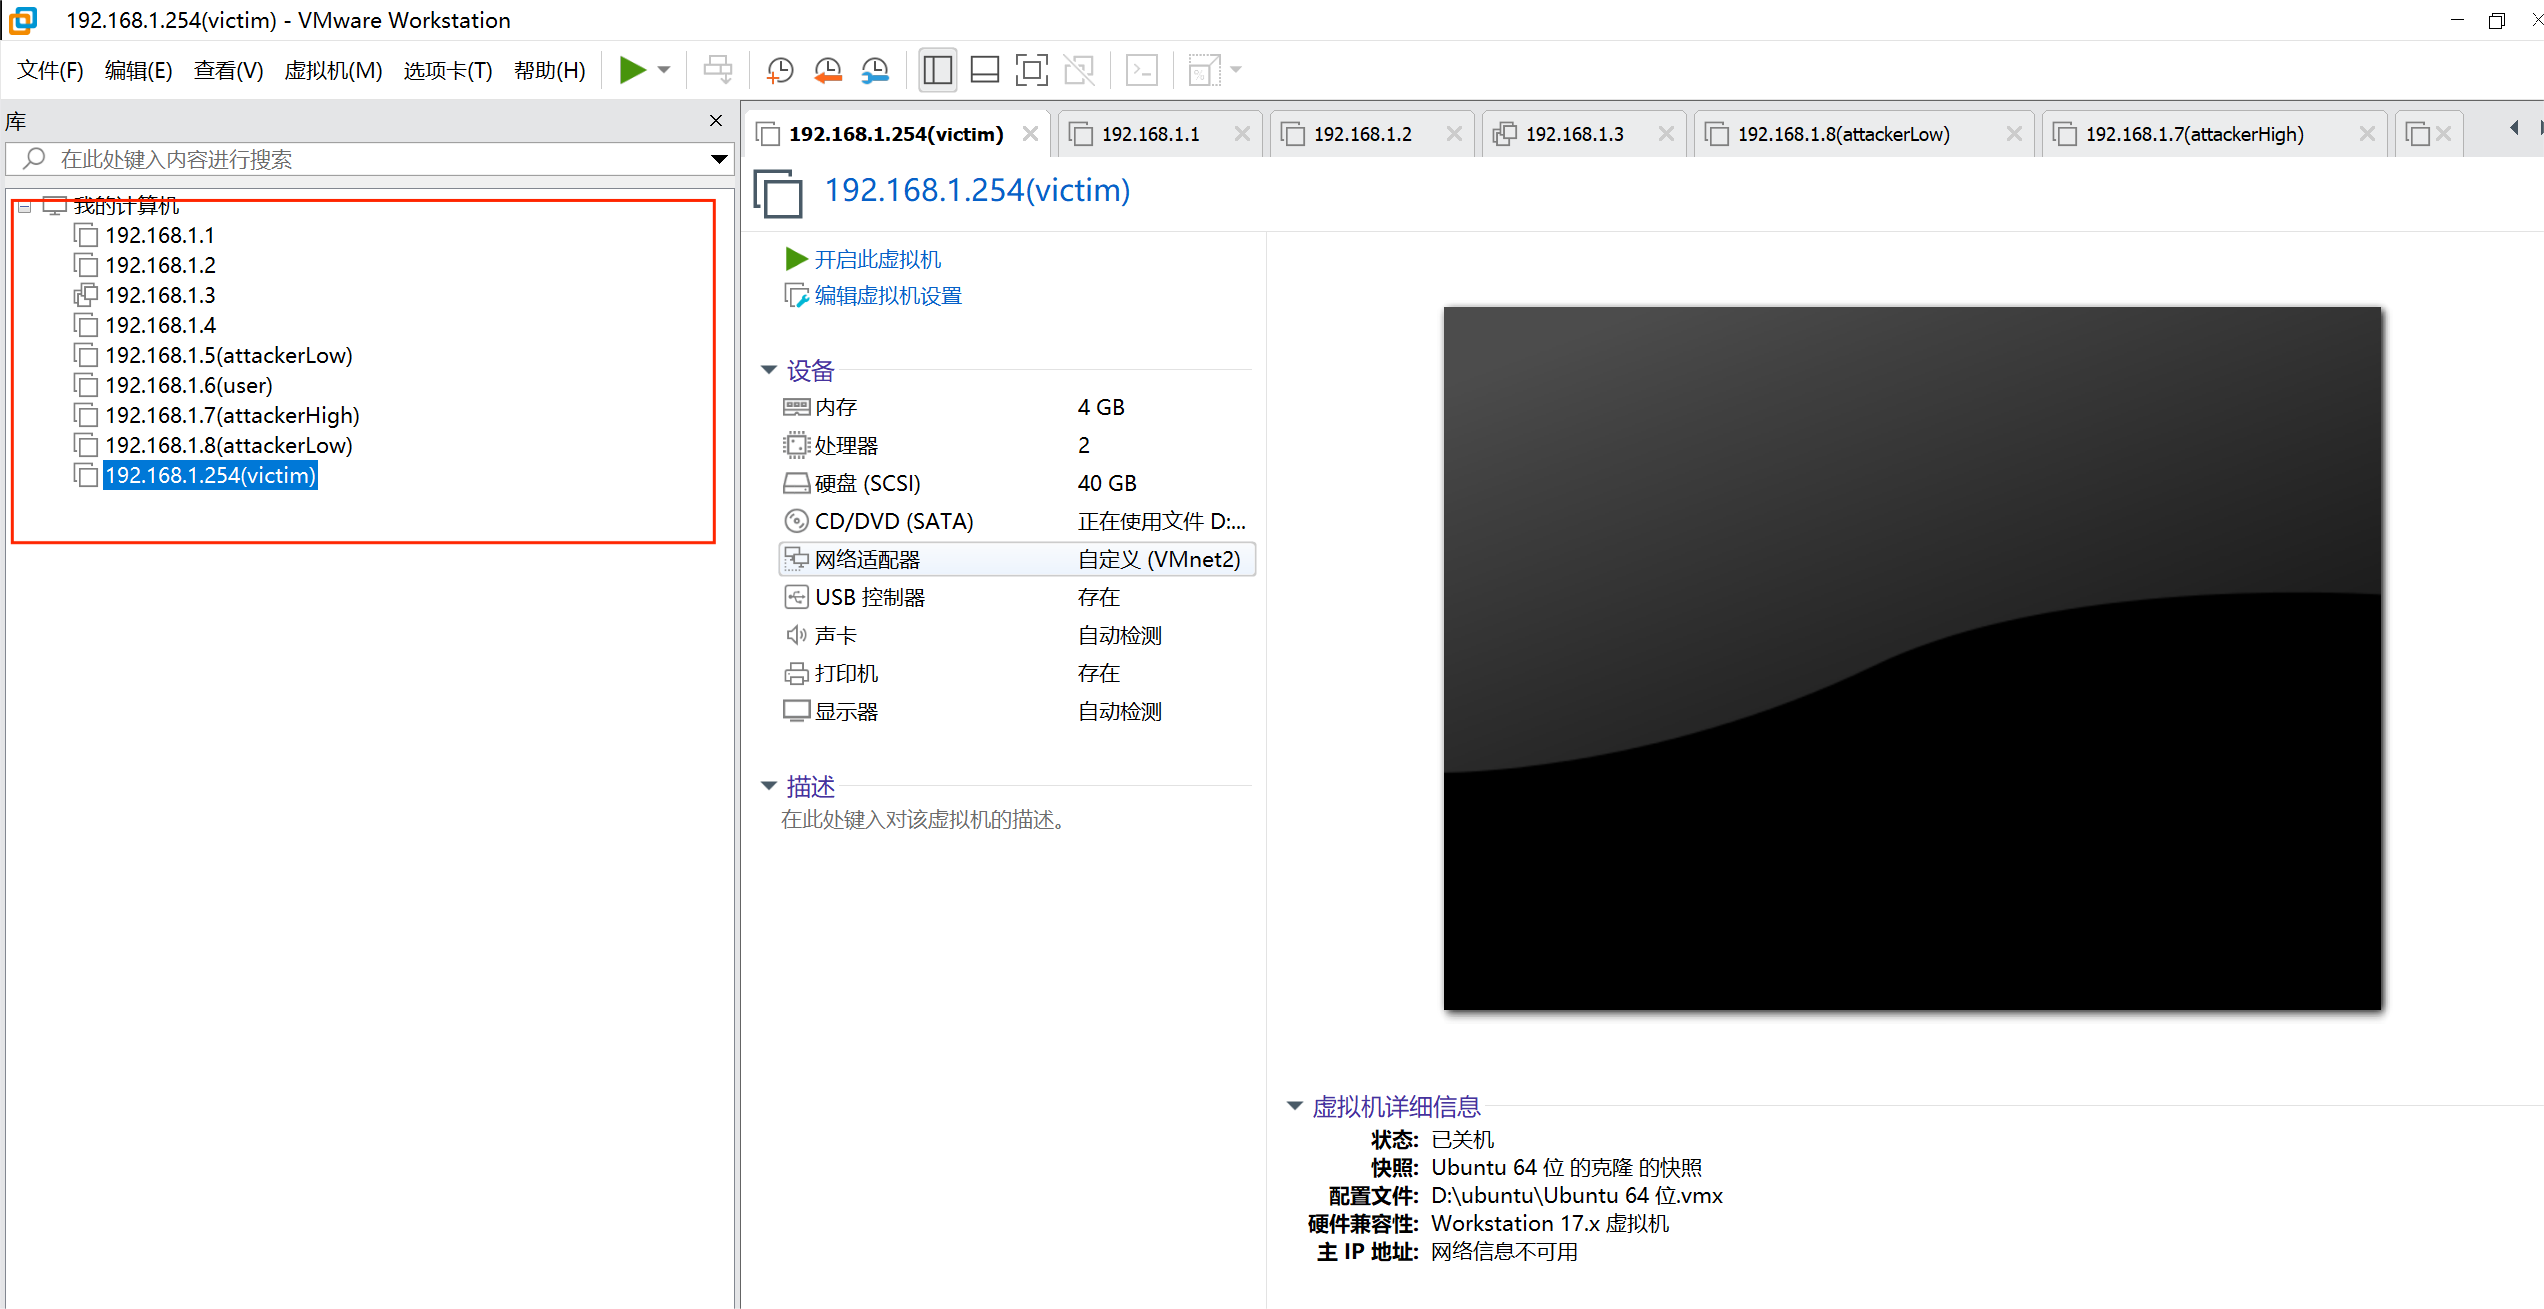
\includegraphics[width=0.9\textwidth]{vmwarelist.png}
	\caption{VMWare 实验虚拟机配置}
	\label{fig:vmwarelist}
\end{figure}
实验中,本文共使用了9台虚拟机,分别扮演不同的角色:一台作为受害者服务器节点,其IP地址为192.168.1.254;四台作为路由转发节点,IP地址依次为192.168.1.1至192.168.1.4;
一台作为高速攻击节点,其IP地址为192.168.1.7;另外两台作为低速攻击节点,IP地址分别为192.168.1.5和192.168.1.8;最后一台作为用户节点,其IP地址为192.168.1.6。\par

图~\ref{fig:vmware_topology}是这些虚拟机构成网络结构的逻辑拓扑图。
\begin{figure}[h]
	\centering
	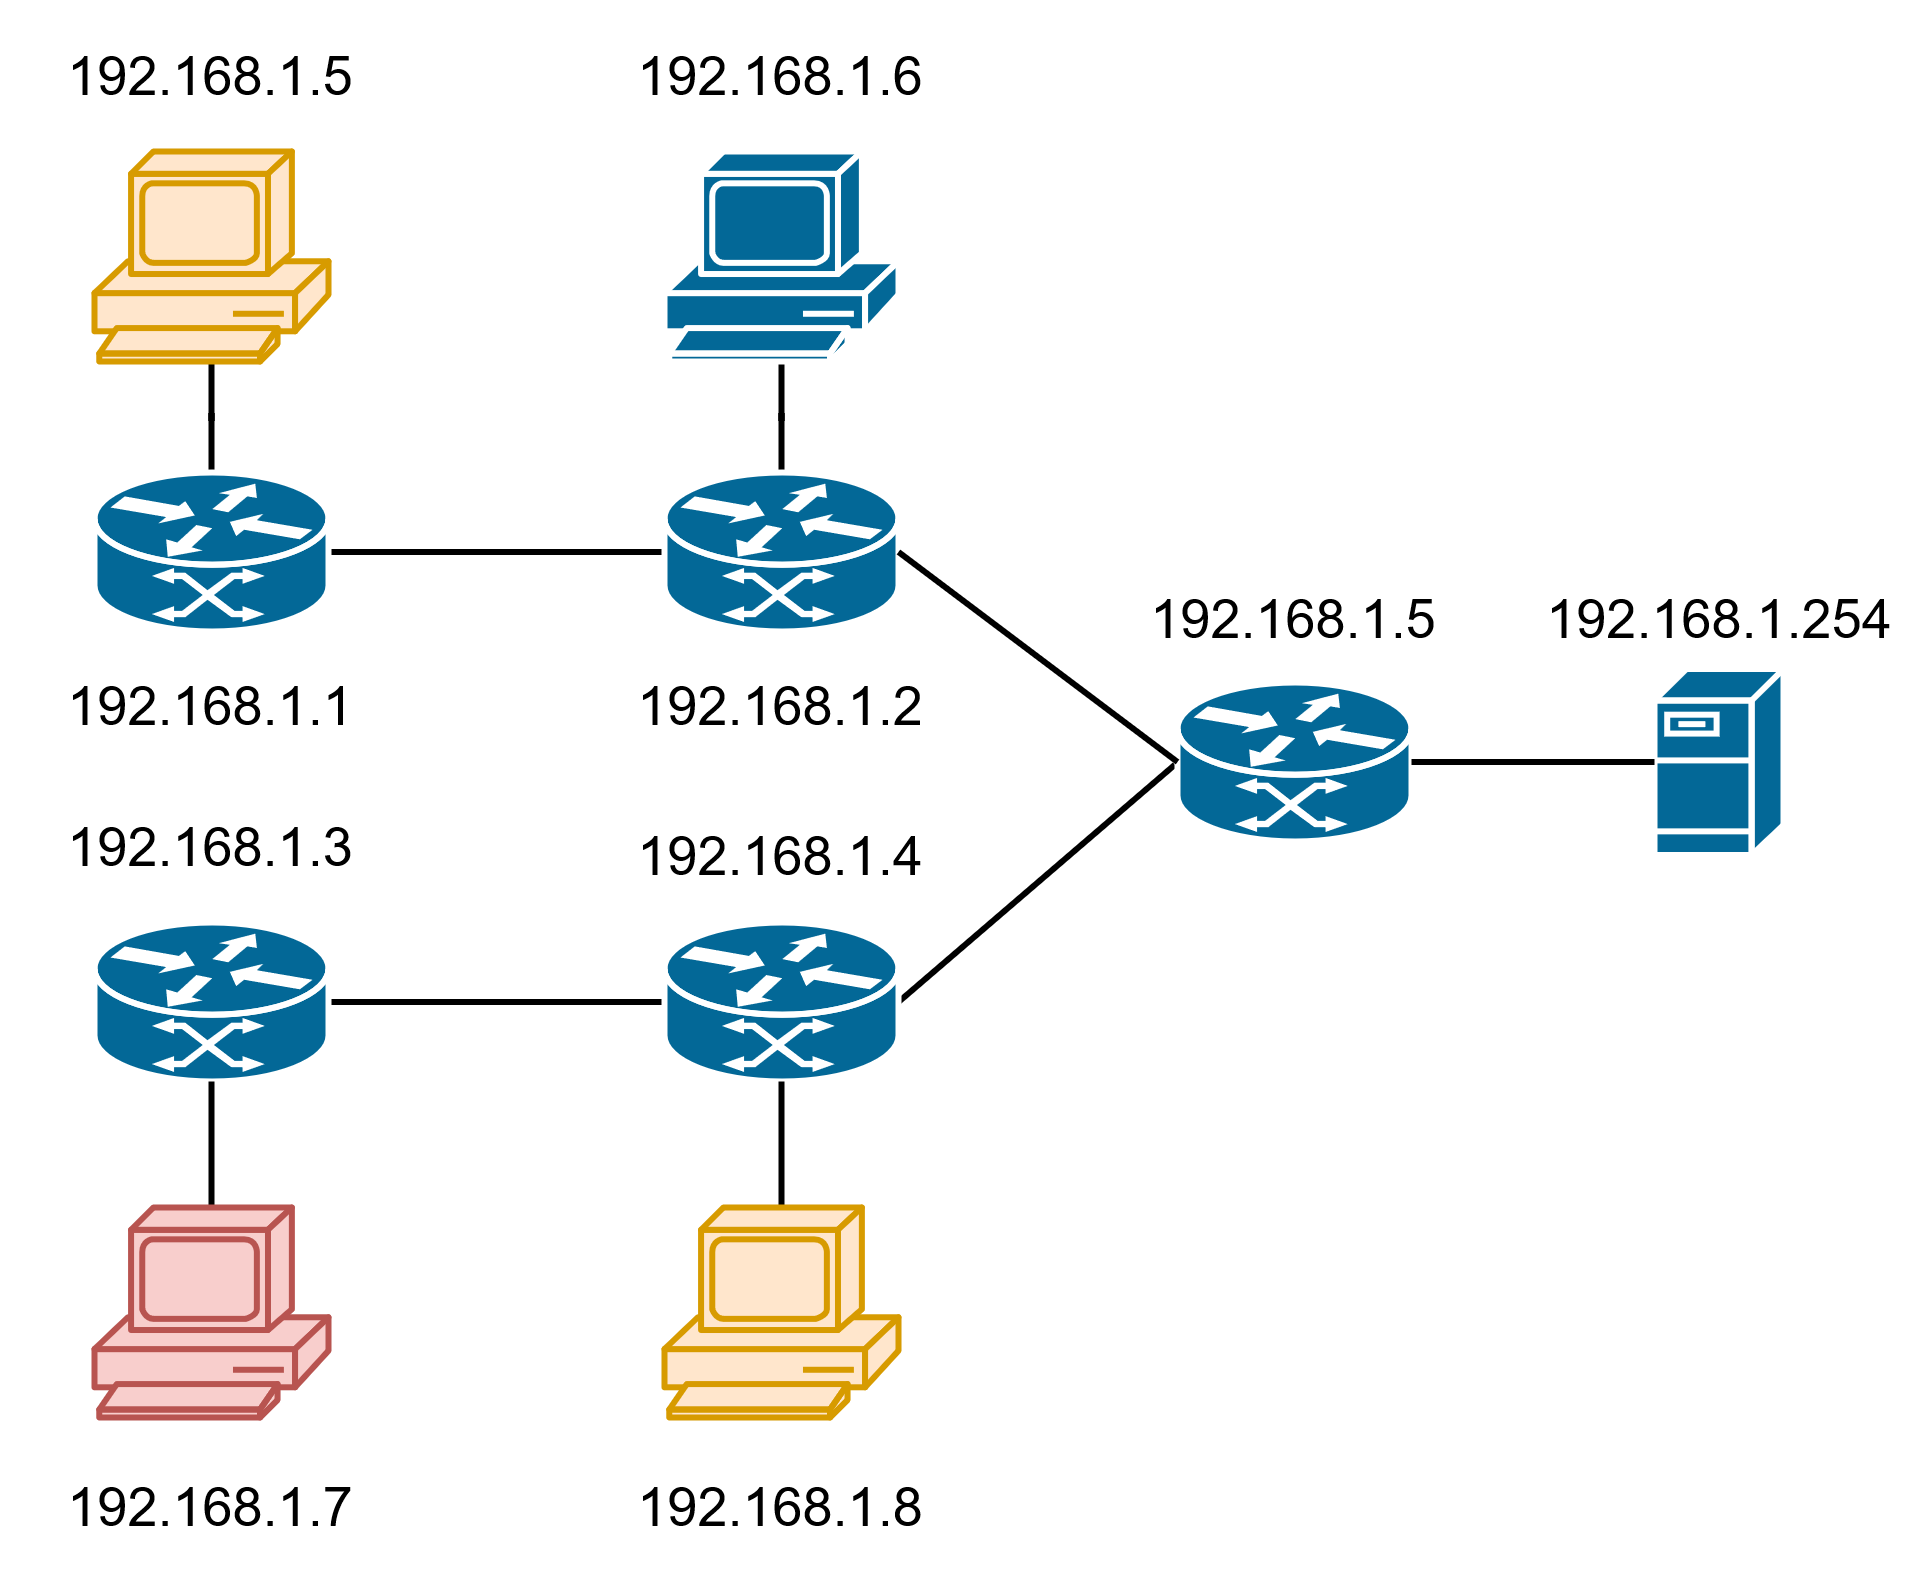
\includegraphics[width=0.6\textwidth]{vmware_topology.drawio.png}
	\caption{VMWare 实验虚拟机逻辑拓扑结构}
	\label{fig:vmware_topology}
\end{figure}
在实验过程中,本文利用Python脚本实现了各项功能。
攻击节点负责发起DoS攻击,其中高速攻击节点不限制攻击速度,而低速攻击节点则设定为每隔五分钟进行一次攻击。
用户节点则模拟普通用户,通过发送ping请求来测试服务器节点的正常服务响应能力。
所有攻击节点不断变换其数据包的IP地址,以模拟DDoS攻击伪造IP地址的场景。
为模拟路由器的路由功能,本文预先编写好了Python程序,引导数据包按照预定的路径通过中间转发节点。
这些转发节点不仅负责转发流量,还实现了数据包的标记功能以及TTL(生存时间)的计算。
受害者节点负责接收数据包,并构建TCP会话以供模型进行检测。
一旦检测成功并触发预警机制,便设定一个阈值(本实验中设为200)。
当某个中间转发节点的IP被标记次数超过这个阈值时,运行在受害者服务器上的Python程序将自动向相关转发节点发送通知消息。
一旦中间转发节点上的Python程序接收到通知消息,它将立即停止引导流量转发,从而实现了模拟路由器的流量过滤功能。
60分钟后,观测实验环境的运行结果。\par

\textbf{2.实验结果分析}\par
图~\ref{fig:attack_rate}~是受害者节点累计所受攻击次数的变化趋势。
\begin{figure}[h]
	\centering
	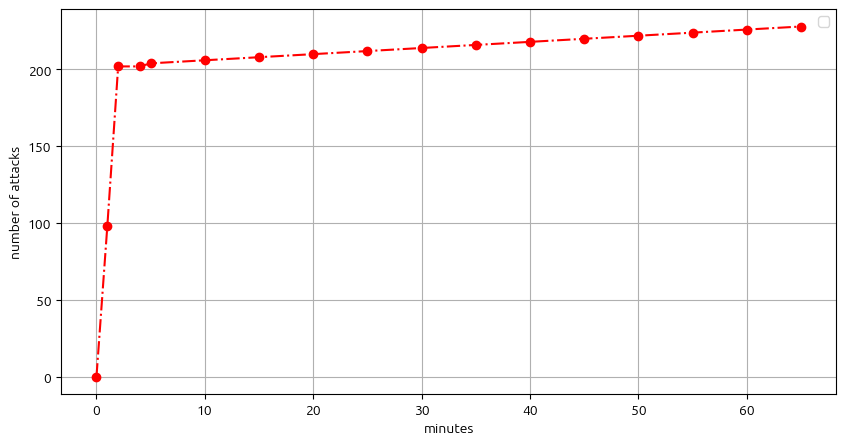
\includegraphics[width=0.7\textwidth]{attack_rate.png}
	\caption{受害者节点累计攻击次数曲线图}
	\label{fig:attack_rate}
\end{figure}
在实验的初始阶段,由于高速攻击节点的持续高强度攻击,服务器所受攻击次数迅速攀升。
然而,当攻击次数触及预设的阈值(200次)后,攻击次数的增长明显放缓。
这一变化表明,高速攻击节点的最近邻路由器因被频繁溯源而触发了防护机制,从而被成功定位并过滤了攻击流量。
随后,实验进入了低速攻击阶段。
低速攻击节点每隔5分钟发起一次攻击,使得服务器每分钟遭受的攻击次数在保持相对稳定的同时呈现出缓慢上升的趋势。
表~\ref{tab:network_status}~是实验环境运行60分钟后,各个发送节点到受害者服务器节点的连通情况。
\begin{table}[h]
	\caption{发送节点到服务器节点的连通情况}
	\label{tab:network_status}
	\centering
	\begin{tabular}{ccccc}
		\toprule
		{\heiti IP} & {\heiti 192.168.1.5} & {\heiti 192.168.1.6} & {\heiti 192.168.1.7} & {\heiti 192.168.1.8} \\
		\midrule
		            & 连通                 & 连通                 & 不连通               & 连通                 \\
		\bottomrule
	\end{tabular}
\end{table}
可以看到此时,高速攻击节点发送的流量已经被路由器过滤掉,而对于低速节点由于攻击频率没有超过阈值而未被过滤,以避免因为低流量的攻击而过滤此路由器上所有访问服务器节点的用户流量,得不偿失。
因此可以得出结论,本文所提出的方案相比PPM方案以及ICMP Ping在面对大规模的网络攻击时具有更高的溯源准确率。

\section{基于溯源的模型防护方法}
\subsection{方法设计}
上文已详细阐述了基于路由器接口号成组标记溯源方法的具体内容,并通过实验验证了其在溯源方面的表现效果。
接下来,本文将在此基础上设计检测模型的防护方法。\par
图~\ref{fig:defend_procedure}~是该方法的具体操作流程。
\begin{figure}[h]
	\centering
	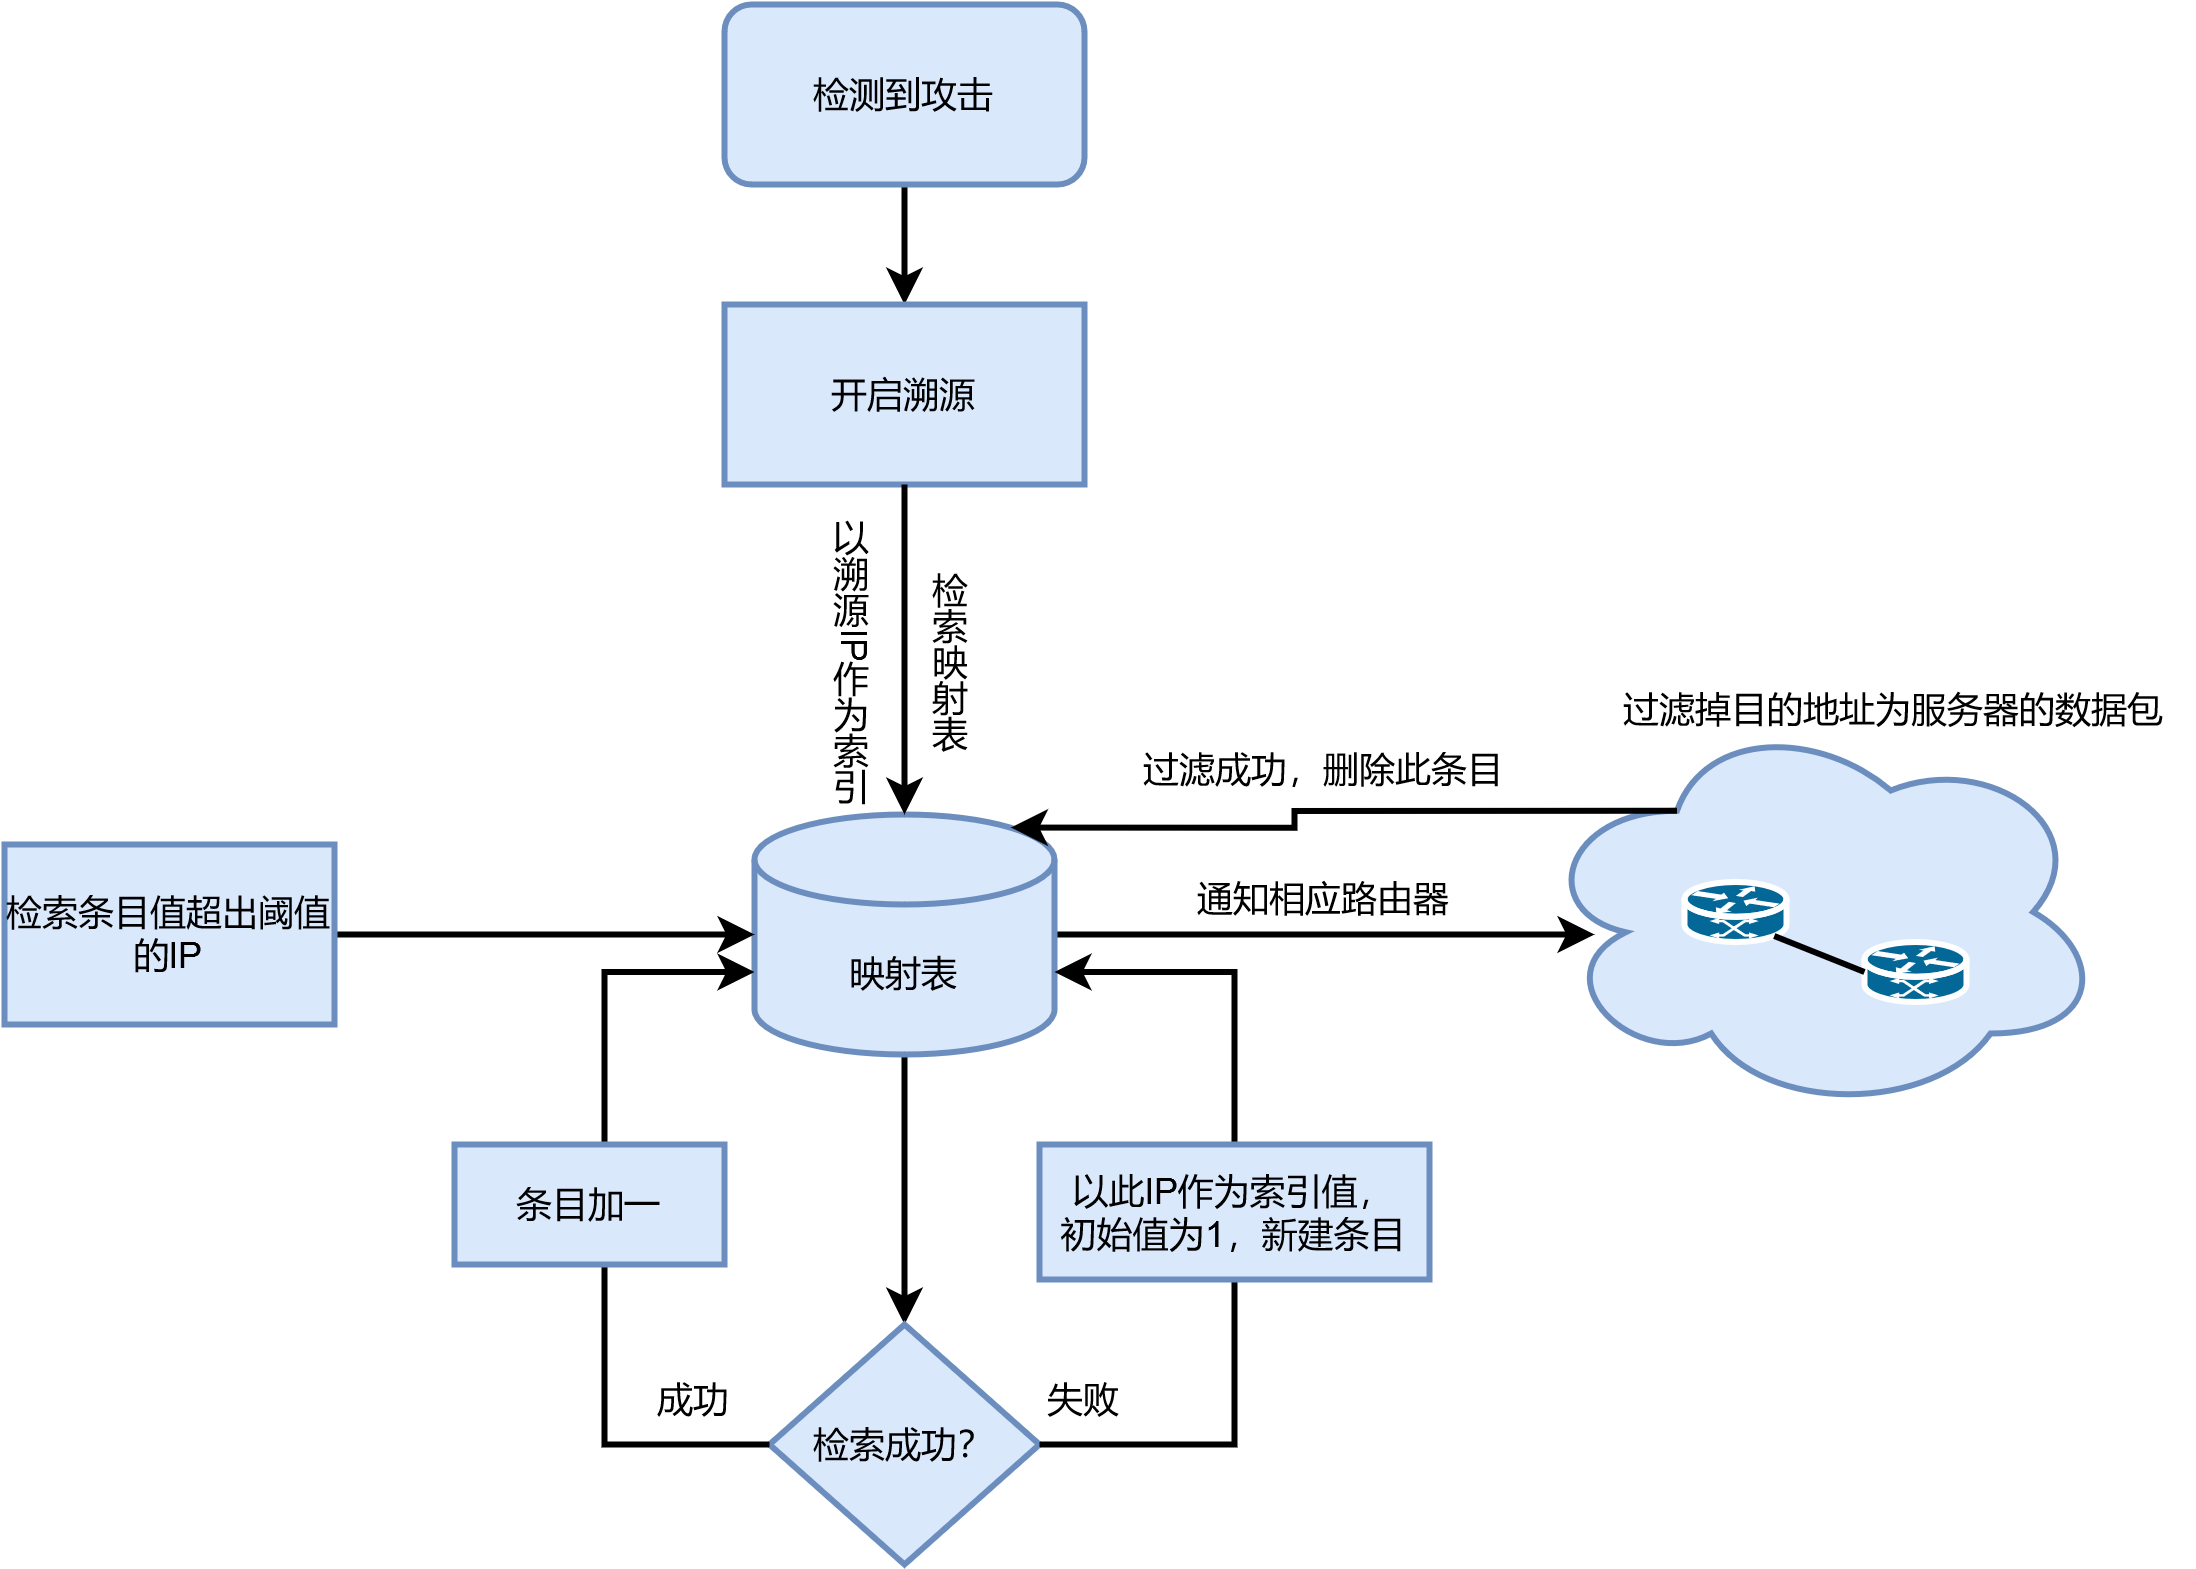
\includegraphics[width=\textwidth]{defend_method.drawio.png}
	\caption{防护流程}
	\label{fig:defend_procedure}
\end{figure}
首先,当检测模型成功检测到攻击流量后,会立即启动溯源机制进行溯源取得溯源结果。
随后,利用溯源结果——即攻击者最近邻的路由器IP作为索引,在映射表中检索对应条目。
其中,映射表是一个用于存储路由器IP地址与对应标记次数之间映射关系的键值对数组。
在这个数组中,IP地址以字符串形式作为索引或键,而与之对应的标记次数则以整数形式作为值。
若在映射表中能够检索到对应条目,则对该条目值进行累加,以实时追踪攻击次数的增长。
若在映射表中不能检索到对应条目,则立即新建一条记录,将溯源获取的IP地址设为索引,并初始化其值为1,为后续累加操作做好准备。
最后,定期检查映射表中是否存在条目值超过预设阈值的情况。
一旦发现有条目值超过阈值,立即通知相关路由器过滤掉发送到该服务器的流量,从而大幅减轻攻击源对检测模型的负担,确保服务器的安全稳定运行。


\subsection{实验评估与分析}
\textbf{1.实验设计}\par
为验证本防护方法的有效性,本文利用VMWare WorkStation构建了一个高度仿真的网络攻击环境,以模拟真实世界中可能遭遇的网络威胁。
图~\ref{fig:vmwarelist}~展示了在VMWare中部署的全部虚拟机列表,所有虚拟机均使用VMnet2网络适配器,确保它们处于同一网络中,从而能够模拟出真实的网络环境。
\begin{figure}[h]
	\centering
	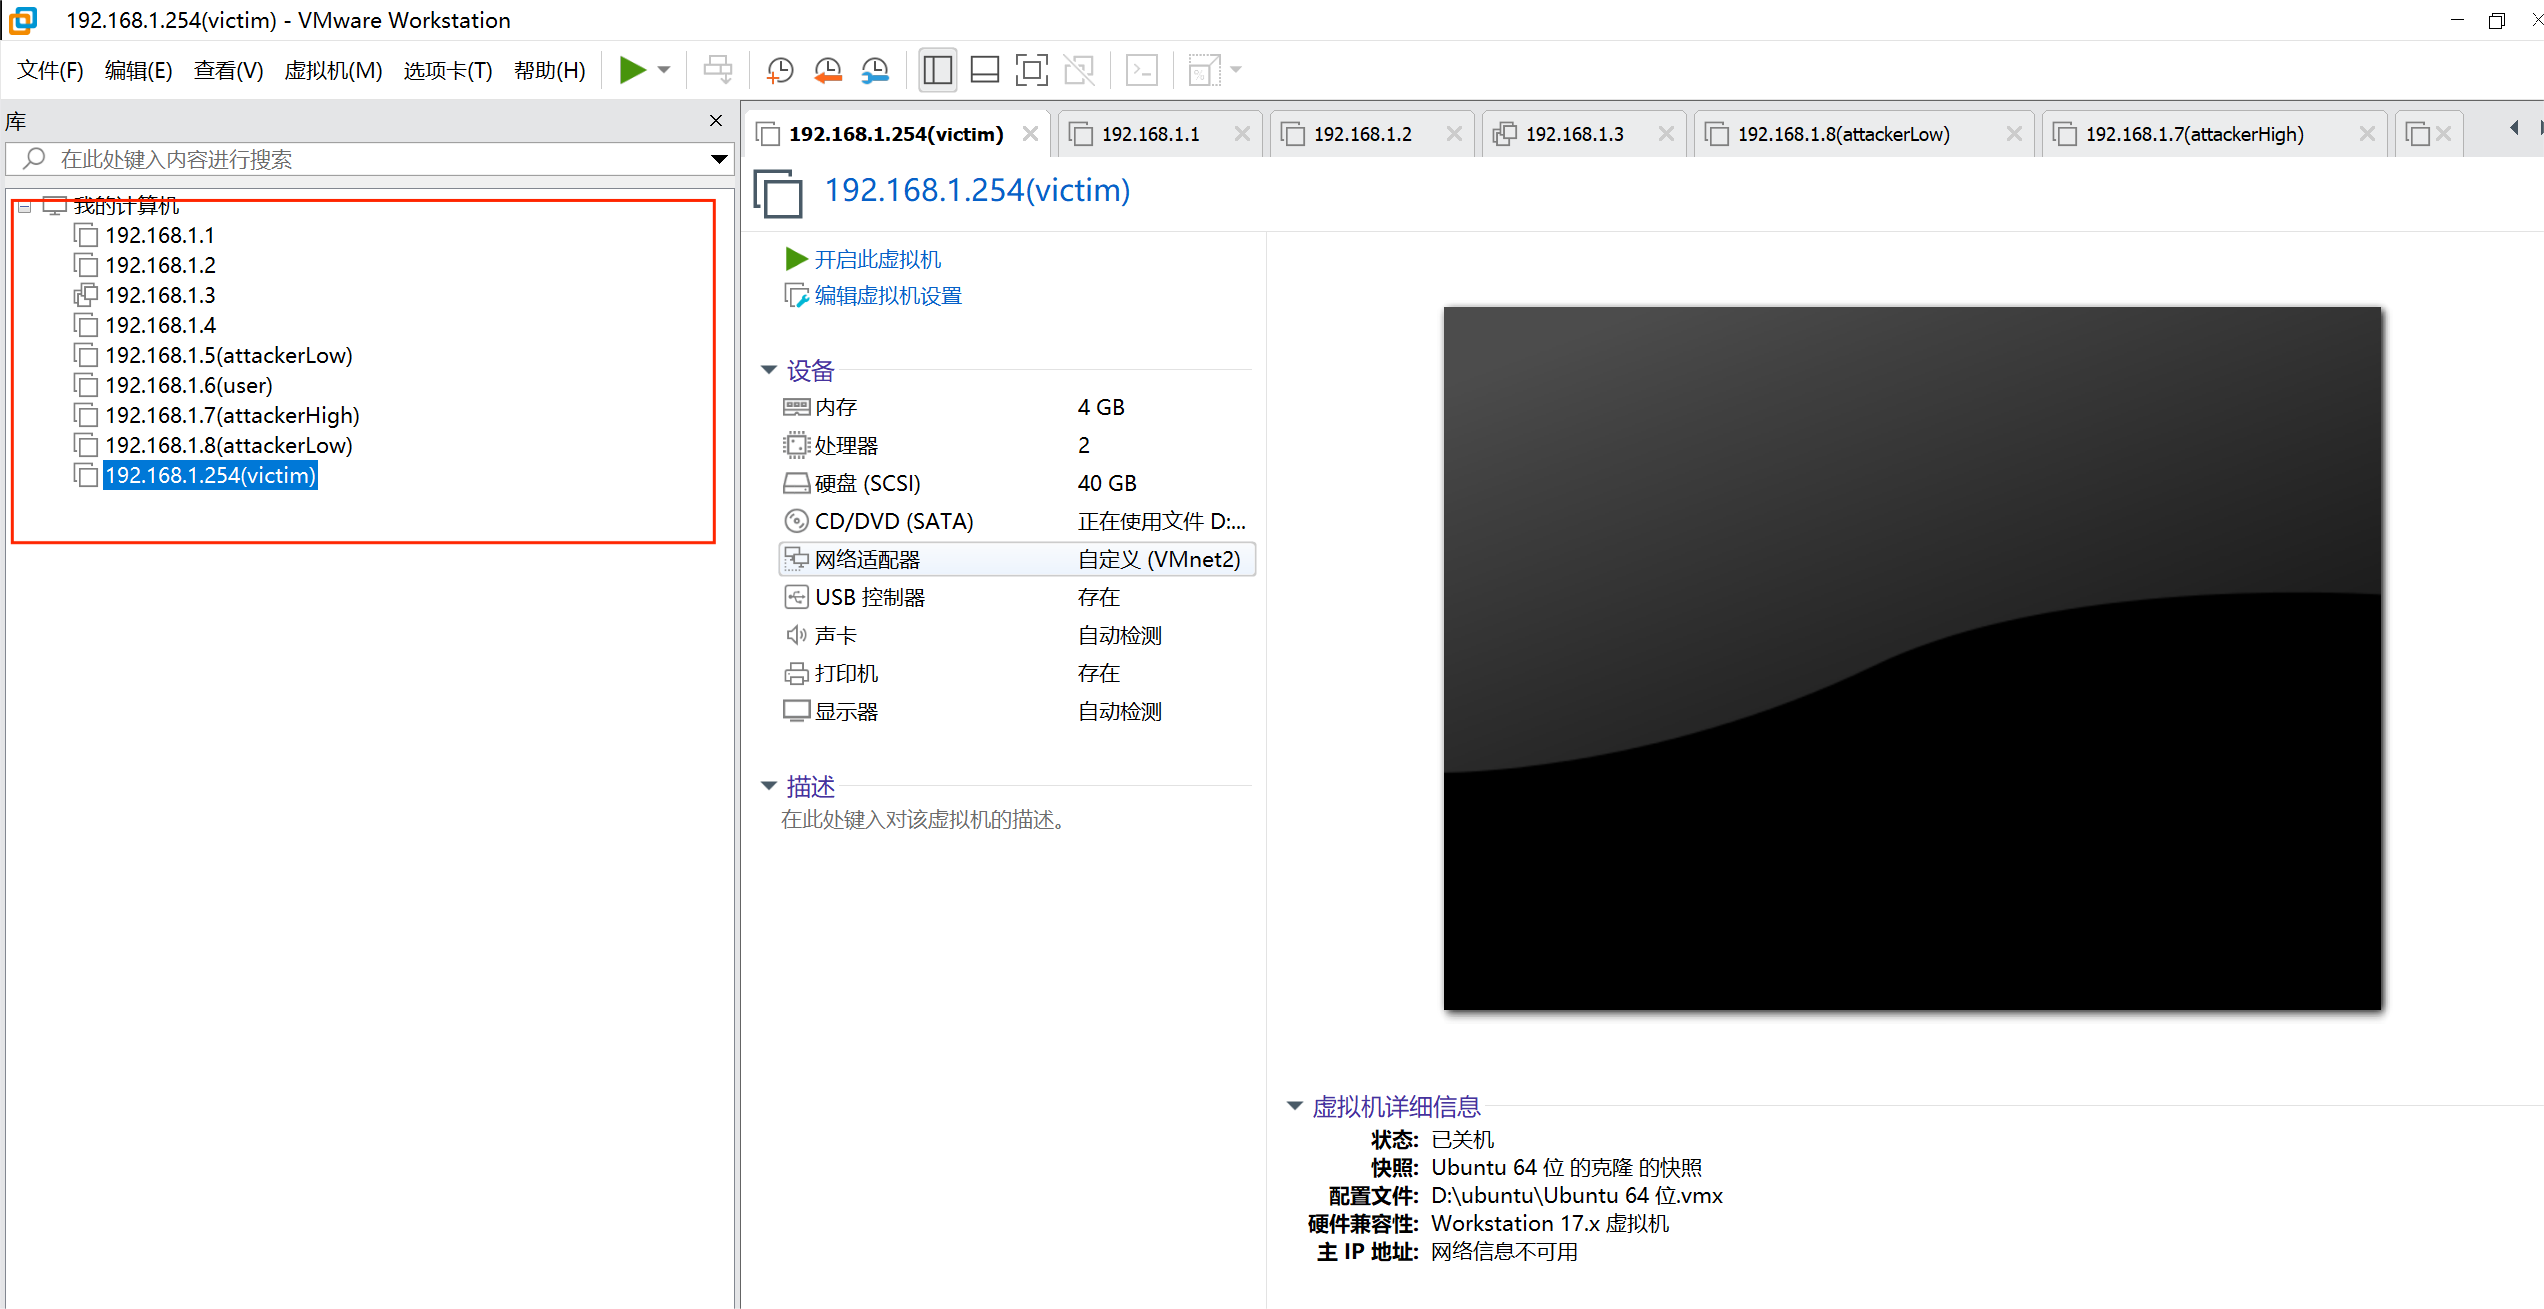
\includegraphics[width=0.9\textwidth]{vmwarelist.png}
	\caption{VMWare 实验虚拟机配置}
	\label{fig:vmwarelist}
\end{figure}
实验中,本文共使用了9台虚拟机,分别扮演不同的角色:一台作为受害者服务器节点,其IP地址为192.168.1.254;四台作为路由转发节点,IP地址依次为192.168.1.1至192.168.1.4;
一台作为高速攻击节点,其IP地址为192.168.1.7;另外两台作为低速攻击节点,IP地址分别为192.168.1.5和192.168.1.8;最后一台作为用户节点,其IP地址为192.168.1.6。\par

图~\ref{fig:vmware_topology}是这些虚拟机构成网络结构的逻辑拓扑图。
\begin{figure}[h]
	\centering
	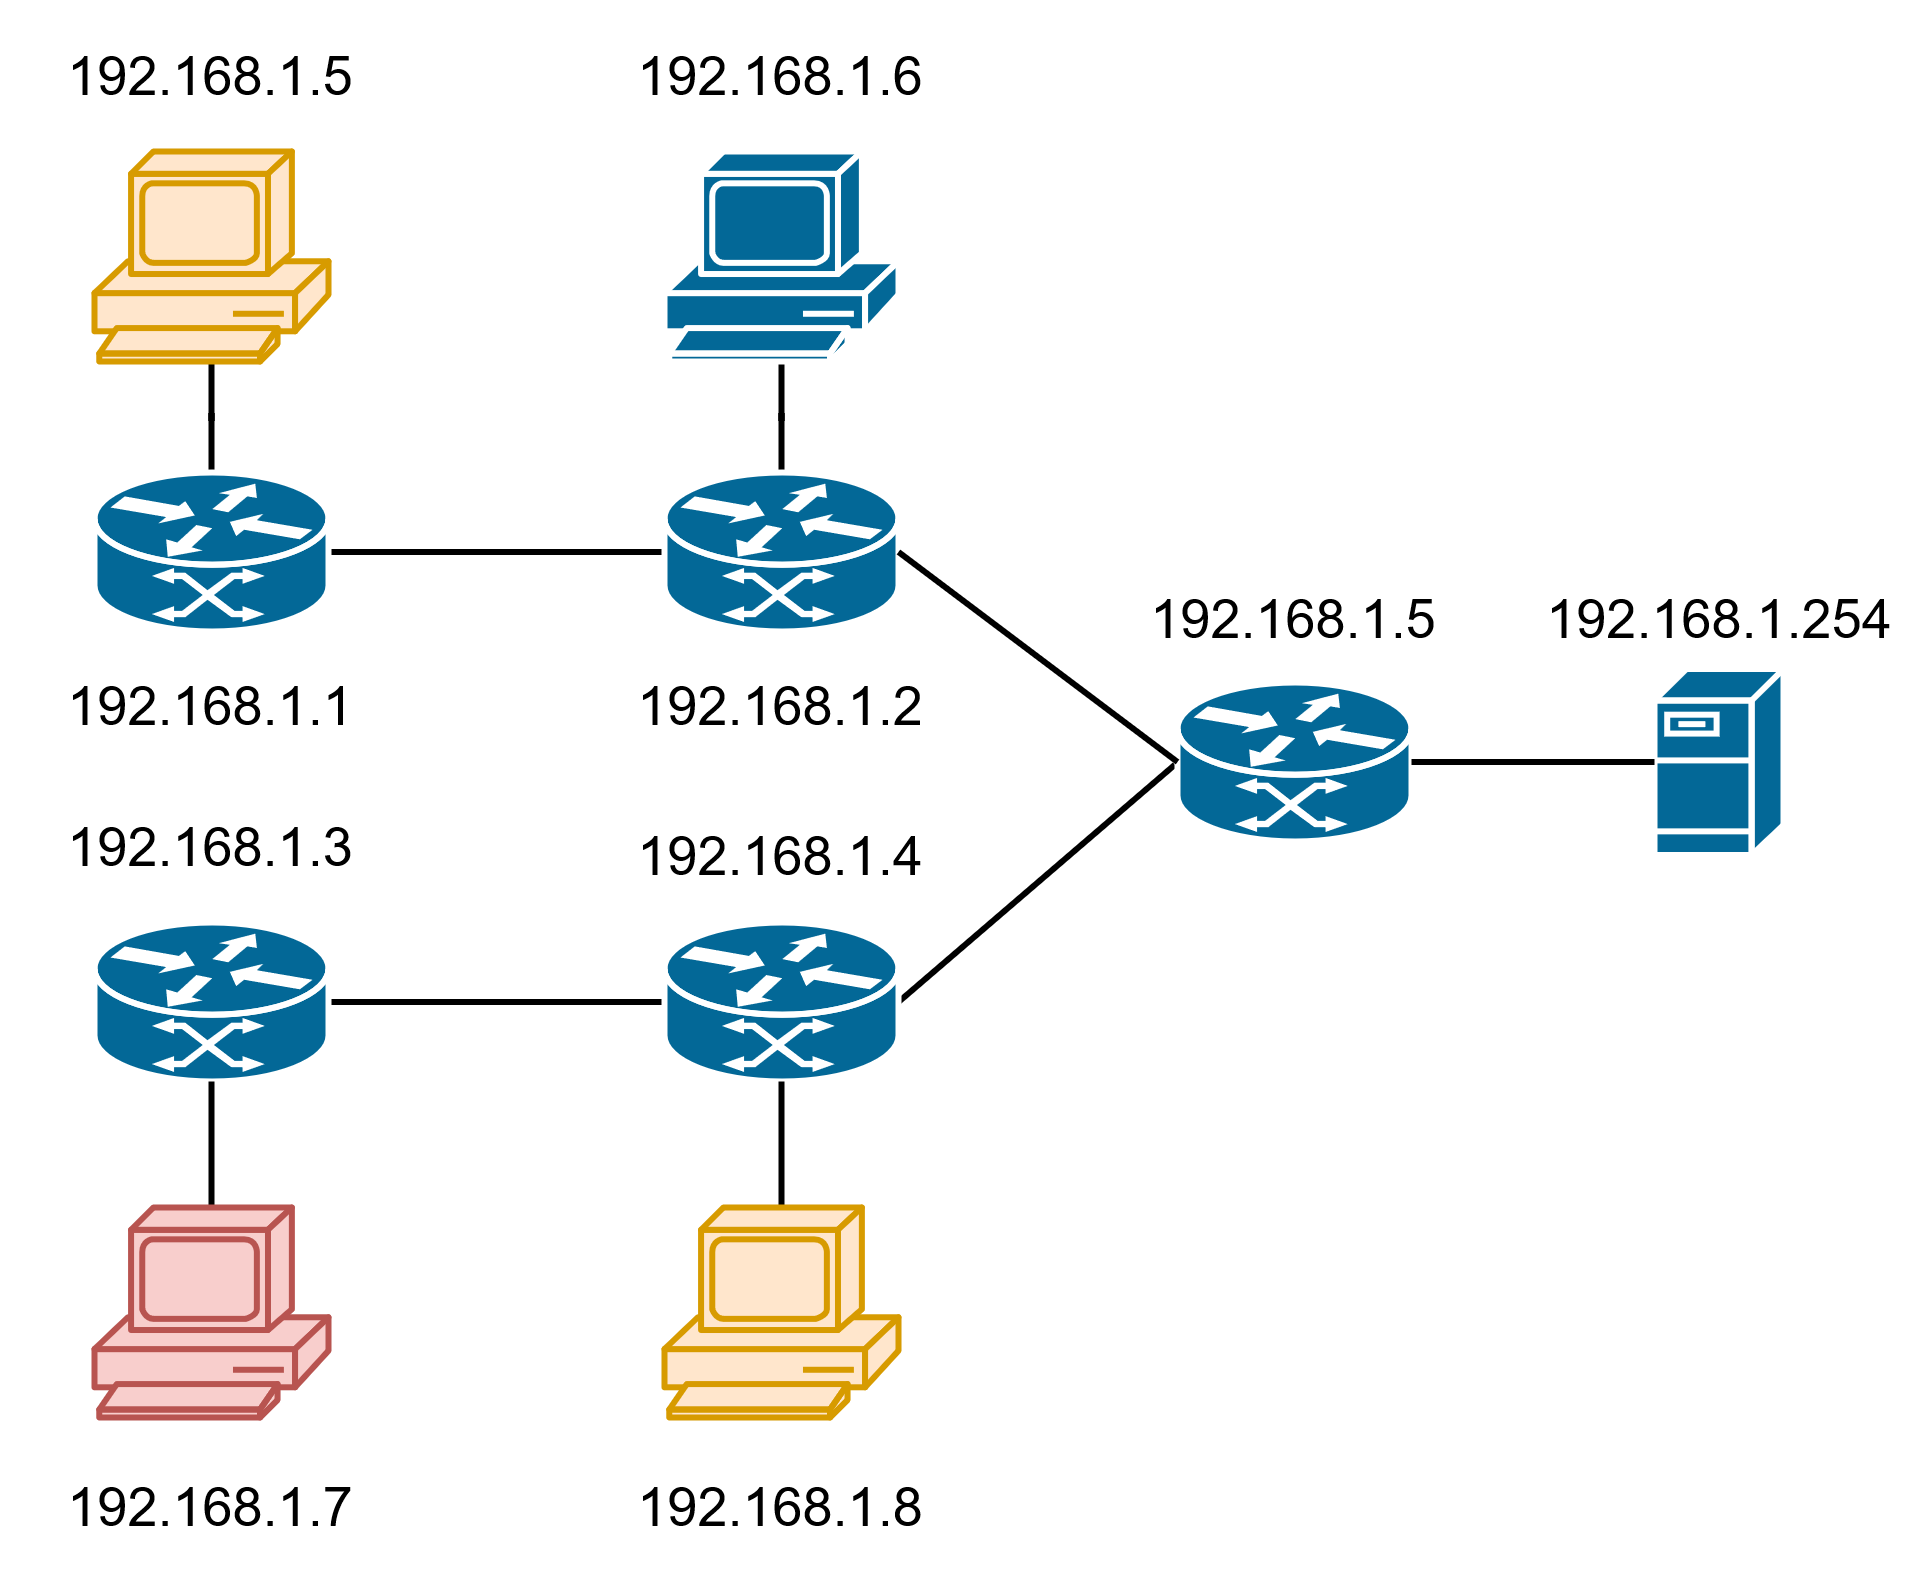
\includegraphics[width=0.6\textwidth]{vmware_topology.drawio.png}
	\caption{VMWare 实验虚拟机逻辑拓扑结构}
	\label{fig:vmware_topology}
\end{figure}
在实验过程中,本文利用Python脚本实现了各项功能。
攻击节点负责发起DoS攻击,其中高速攻击节点不限制攻击速度,而低速攻击节点则设定为每隔五分钟进行一次攻击。
用户节点则模拟普通用户,通过发送ping请求来测试服务器节点的正常服务响应能力。
所有攻击节点不断变换其数据包的IP地址,以模拟DDoS攻击伪造IP地址的场景。
为模拟路由器的路由功能,本文预先编写好了Python程序,引导数据包按照预定的路径通过中间转发节点。
这些转发节点不仅负责转发流量,还实现了数据包的标记功能以及TTL(生存时间)的计算。
受害者节点负责接收数据包,并构建TCP会话以供模型进行检测。
一旦检测成功并触发预警机制,便设定一个阈值(本实验中设为200)。
当某个中间转发节点的IP被标记次数超过这个阈值时,运行在受害者服务器上的Python程序将自动向相关转发节点发送通知消息。
一旦中间转发节点上的Python程序接收到通知消息,它将立即停止引导流量转发,从而实现了模拟路由器的流量过滤功能。
60分钟后,观测实验环境的运行结果。\par

\textbf{2.实验结果分析}\par
图~\ref{fig:attack_rate}~是受害者节点累计所受攻击次数的变化趋势。
\begin{figure}[h]
	\centering
	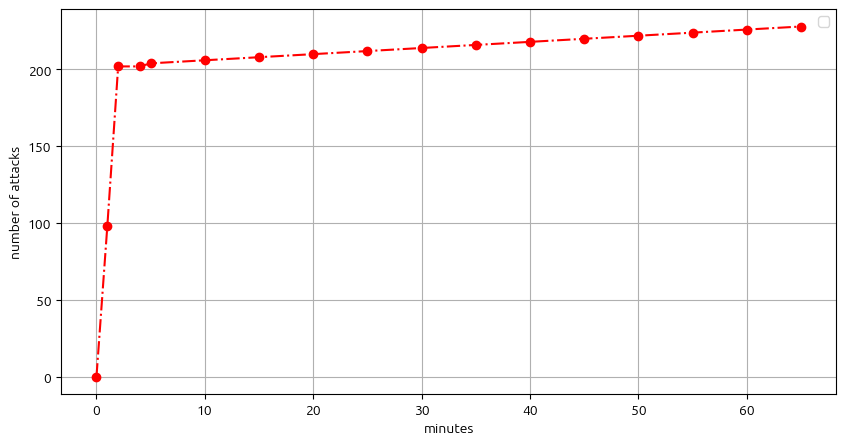
\includegraphics[width=0.7\textwidth]{attack_rate.png}
	\caption{受害者节点累计攻击次数曲线图}
	\label{fig:attack_rate}
\end{figure}
在实验的初始阶段,由于高速攻击节点的持续高强度攻击,服务器所受攻击次数迅速攀升。
然而,当攻击次数触及预设的阈值(200次)后,攻击次数的增长明显放缓。
这一变化表明,高速攻击节点的最近邻路由器因被频繁溯源而触发了防护机制,从而被成功定位并过滤了攻击流量。
随后,实验进入了低速攻击阶段。
低速攻击节点每隔5分钟发起一次攻击,使得服务器每分钟遭受的攻击次数在保持相对稳定的同时呈现出缓慢上升的趋势。
表~\ref{tab:network_status}~是实验环境运行60分钟后,各个发送节点到受害者服务器节点的连通情况。
\begin{table}[h]
	\caption{发送节点到服务器节点的连通情况}
	\label{tab:network_status}
	\centering
	\begin{tabular}{ccccc}
		\toprule
		{\heiti IP} & {\heiti 192.168.1.5} & {\heiti 192.168.1.6} & {\heiti 192.168.1.7} & {\heiti 192.168.1.8} \\
		\midrule
		            & 连通                 & 连通                 & 不连通               & 连通                 \\
		\bottomrule
	\end{tabular}
\end{table}
可以看到此时,高速攻击节点发送的流量已经被路由器过滤掉,而对于低速节点由于攻击频率没有超过阈值而未被过滤,以避免因为低流量的攻击而过滤此路由器上所有访问服务器节点的用户流量,得不偿失。
\section{本章小结}
本章提出了一种基于溯源的异常流量检测模型防护方法,旨在解决DDoS攻击导致的模型负担过重问题。
该防护方法的核心在于采用改进的数据包标记溯源技术,通过基于路由器接口号成组的标记方式,实现了高效且准确的流量溯源。为此,本章首先详细描述了该溯源方法的流程及原理,并通过实验验证其性能。
实验结果表明,与PPM方法相比,本方法在溯源速度和准确率上均展现出显著优势。
随后,本章进一步阐述了所提防护方法的整体流程,并在高度仿真的网络攻击环境中进行了实际测试。
测试结果表明,该方法能有效定位并过滤攻击流量,从而确保异常流量检测模型及服务器的稳定运行。
本章提出了一种基于溯源的异常流量检测模型防护方法,旨在解决DDoS攻击导致的模型负担过重问题。
该防护方法的核心在于采用改进的数据包标记溯源技术,通过基于路由器接口号成组的标记方式,实现了高效且准确的流量溯源。为此,本章首先详细描述了该溯源方法的流程及原理,并通过实验验证其性能。
实验结果表明,与PPM方法相比,本方法在溯源速度和准确率上均展现出显著优势。
随后,本章进一步阐述了所提防护方法的整体流程,并在高度仿真的网络攻击环境中进行了实际测试。
测试结果表明,该方法能有效定位并过滤攻击流量,从而确保异常流量检测模型及服务器的稳定运行。